% Options for packages loaded elsewhere
\PassOptionsToPackage{unicode}{hyperref}
\PassOptionsToPackage{hyphens}{url}
%
\documentclass[
]{article}
\usepackage{amsmath,amssymb}
\usepackage{lmodern}
\usepackage{iftex}
\ifPDFTeX
  \usepackage[T1]{fontenc}
  \usepackage[utf8]{inputenc}
  \usepackage{textcomp} % provide euro and other symbols
\else % if luatex or xetex
  \usepackage{unicode-math}
  \defaultfontfeatures{Scale=MatchLowercase}
  \defaultfontfeatures[\rmfamily]{Ligatures=TeX,Scale=1}
\fi
% Use upquote if available, for straight quotes in verbatim environments
\IfFileExists{upquote.sty}{\usepackage{upquote}}{}
\IfFileExists{microtype.sty}{% use microtype if available
  \usepackage[]{microtype}
  \UseMicrotypeSet[protrusion]{basicmath} % disable protrusion for tt fonts
}{}
\makeatletter
\@ifundefined{KOMAClassName}{% if non-KOMA class
  \IfFileExists{parskip.sty}{%
    \usepackage{parskip}
  }{% else
    \setlength{\parindent}{0pt}
    \setlength{\parskip}{6pt plus 2pt minus 1pt}}
}{% if KOMA class
  \KOMAoptions{parskip=half}}
\makeatother
\usepackage{xcolor}
\usepackage[margin=1in]{geometry}
\usepackage{color}
\usepackage{fancyvrb}
\newcommand{\VerbBar}{|}
\newcommand{\VERB}{\Verb[commandchars=\\\{\}]}
\DefineVerbatimEnvironment{Highlighting}{Verbatim}{commandchars=\\\{\}}
% Add ',fontsize=\small' for more characters per line
\usepackage{framed}
\definecolor{shadecolor}{RGB}{248,248,248}
\newenvironment{Shaded}{\begin{snugshade}}{\end{snugshade}}
\newcommand{\AlertTok}[1]{\textcolor[rgb]{0.94,0.16,0.16}{#1}}
\newcommand{\AnnotationTok}[1]{\textcolor[rgb]{0.56,0.35,0.01}{\textbf{\textit{#1}}}}
\newcommand{\AttributeTok}[1]{\textcolor[rgb]{0.77,0.63,0.00}{#1}}
\newcommand{\BaseNTok}[1]{\textcolor[rgb]{0.00,0.00,0.81}{#1}}
\newcommand{\BuiltInTok}[1]{#1}
\newcommand{\CharTok}[1]{\textcolor[rgb]{0.31,0.60,0.02}{#1}}
\newcommand{\CommentTok}[1]{\textcolor[rgb]{0.56,0.35,0.01}{\textit{#1}}}
\newcommand{\CommentVarTok}[1]{\textcolor[rgb]{0.56,0.35,0.01}{\textbf{\textit{#1}}}}
\newcommand{\ConstantTok}[1]{\textcolor[rgb]{0.00,0.00,0.00}{#1}}
\newcommand{\ControlFlowTok}[1]{\textcolor[rgb]{0.13,0.29,0.53}{\textbf{#1}}}
\newcommand{\DataTypeTok}[1]{\textcolor[rgb]{0.13,0.29,0.53}{#1}}
\newcommand{\DecValTok}[1]{\textcolor[rgb]{0.00,0.00,0.81}{#1}}
\newcommand{\DocumentationTok}[1]{\textcolor[rgb]{0.56,0.35,0.01}{\textbf{\textit{#1}}}}
\newcommand{\ErrorTok}[1]{\textcolor[rgb]{0.64,0.00,0.00}{\textbf{#1}}}
\newcommand{\ExtensionTok}[1]{#1}
\newcommand{\FloatTok}[1]{\textcolor[rgb]{0.00,0.00,0.81}{#1}}
\newcommand{\FunctionTok}[1]{\textcolor[rgb]{0.00,0.00,0.00}{#1}}
\newcommand{\ImportTok}[1]{#1}
\newcommand{\InformationTok}[1]{\textcolor[rgb]{0.56,0.35,0.01}{\textbf{\textit{#1}}}}
\newcommand{\KeywordTok}[1]{\textcolor[rgb]{0.13,0.29,0.53}{\textbf{#1}}}
\newcommand{\NormalTok}[1]{#1}
\newcommand{\OperatorTok}[1]{\textcolor[rgb]{0.81,0.36,0.00}{\textbf{#1}}}
\newcommand{\OtherTok}[1]{\textcolor[rgb]{0.56,0.35,0.01}{#1}}
\newcommand{\PreprocessorTok}[1]{\textcolor[rgb]{0.56,0.35,0.01}{\textit{#1}}}
\newcommand{\RegionMarkerTok}[1]{#1}
\newcommand{\SpecialCharTok}[1]{\textcolor[rgb]{0.00,0.00,0.00}{#1}}
\newcommand{\SpecialStringTok}[1]{\textcolor[rgb]{0.31,0.60,0.02}{#1}}
\newcommand{\StringTok}[1]{\textcolor[rgb]{0.31,0.60,0.02}{#1}}
\newcommand{\VariableTok}[1]{\textcolor[rgb]{0.00,0.00,0.00}{#1}}
\newcommand{\VerbatimStringTok}[1]{\textcolor[rgb]{0.31,0.60,0.02}{#1}}
\newcommand{\WarningTok}[1]{\textcolor[rgb]{0.56,0.35,0.01}{\textbf{\textit{#1}}}}
\usepackage{graphicx}
\makeatletter
\def\maxwidth{\ifdim\Gin@nat@width>\linewidth\linewidth\else\Gin@nat@width\fi}
\def\maxheight{\ifdim\Gin@nat@height>\textheight\textheight\else\Gin@nat@height\fi}
\makeatother
% Scale images if necessary, so that they will not overflow the page
% margins by default, and it is still possible to overwrite the defaults
% using explicit options in \includegraphics[width, height, ...]{}
\setkeys{Gin}{width=\maxwidth,height=\maxheight,keepaspectratio}
% Set default figure placement to htbp
\makeatletter
\def\fps@figure{htbp}
\makeatother
\setlength{\emergencystretch}{3em} % prevent overfull lines
\providecommand{\tightlist}{%
  \setlength{\itemsep}{0pt}\setlength{\parskip}{0pt}}
\setcounter{secnumdepth}{-\maxdimen} % remove section numbering
\ifLuaTeX
  \usepackage{selnolig}  % disable illegal ligatures
\fi
\IfFileExists{bookmark.sty}{\usepackage{bookmark}}{\usepackage{hyperref}}
\IfFileExists{xurl.sty}{\usepackage{xurl}}{} % add URL line breaks if available
\urlstyle{same} % disable monospaced font for URLs
\hypersetup{
  pdftitle={Data 583 Life Expectancy (WHO)},
  pdfauthor={Justin Chan, Kenny Tong, Viji Rajagopalan},
  hidelinks,
  pdfcreator={LaTeX via pandoc}}

\title{Data 583 Life Expectancy (WHO)}
\author{Justin Chan, Kenny Tong, Viji Rajagopalan}
\date{7 Mar, 2023}

\begin{document}
\maketitle

\hypertarget{eda}{%
\subsection{EDA}\label{eda}}

\hypertarget{original-dataset-summary-initial-data-screening}{%
\subsubsection{Original Dataset Summary \& Initial Data
Screening}\label{original-dataset-summary-initial-data-screening}}

Purpose : Let's take a snapshot of the original dataset and have a rough
idea of its record

\begin{Shaded}
\begin{Highlighting}[]
\NormalTok{le }\OtherTok{\textless{}{-}} \FunctionTok{read.csv}\NormalTok{(}\StringTok{"dataset/LifeExpectancy.csv"}\NormalTok{)}
\FunctionTok{summary}\NormalTok{(le)}
\end{Highlighting}
\end{Shaded}

\begin{verbatim}
##    Country               Year         Status          Life.expectancy
##  Length:2938        Min.   :2000   Length:2938        Min.   :36.30  
##  Class :character   1st Qu.:2004   Class :character   1st Qu.:63.10  
##  Mode  :character   Median :2008   Mode  :character   Median :72.10  
##                     Mean   :2008                      Mean   :69.22  
##                     3rd Qu.:2012                      3rd Qu.:75.70  
##                     Max.   :2015                      Max.   :89.00  
##                                                       NA's   :10     
##  Adult.Mortality infant.deaths       Alcohol        percentage.expenditure
##  Min.   :  1.0   Min.   :   0.0   Min.   : 0.0100   Min.   :    0.000     
##  1st Qu.: 74.0   1st Qu.:   0.0   1st Qu.: 0.8775   1st Qu.:    4.685     
##  Median :144.0   Median :   3.0   Median : 3.7550   Median :   64.913     
##  Mean   :164.8   Mean   :  30.3   Mean   : 4.6029   Mean   :  738.251     
##  3rd Qu.:228.0   3rd Qu.:  22.0   3rd Qu.: 7.7025   3rd Qu.:  441.534     
##  Max.   :723.0   Max.   :1800.0   Max.   :17.8700   Max.   :19479.912     
##  NA's   :10                       NA's   :194                             
##   Hepatitis.B       Measles              BMI        under.five.deaths
##  Min.   : 1.00   Min.   :     0.0   Min.   : 1.00   Min.   :   0.00  
##  1st Qu.:77.00   1st Qu.:     0.0   1st Qu.:19.30   1st Qu.:   0.00  
##  Median :92.00   Median :    17.0   Median :43.50   Median :   4.00  
##  Mean   :80.94   Mean   :  2419.6   Mean   :38.32   Mean   :  42.04  
##  3rd Qu.:97.00   3rd Qu.:   360.2   3rd Qu.:56.20   3rd Qu.:  28.00  
##  Max.   :99.00   Max.   :212183.0   Max.   :87.30   Max.   :2500.00  
##  NA's   :553                        NA's   :34                       
##      Polio       Total.expenditure   Diphtheria       HIV.AIDS     
##  Min.   : 3.00   Min.   : 0.370    Min.   : 2.00   Min.   : 0.100  
##  1st Qu.:78.00   1st Qu.: 4.260    1st Qu.:78.00   1st Qu.: 0.100  
##  Median :93.00   Median : 5.755    Median :93.00   Median : 0.100  
##  Mean   :82.55   Mean   : 5.938    Mean   :82.32   Mean   : 1.742  
##  3rd Qu.:97.00   3rd Qu.: 7.492    3rd Qu.:97.00   3rd Qu.: 0.800  
##  Max.   :99.00   Max.   :17.600    Max.   :99.00   Max.   :50.600  
##  NA's   :19      NA's   :226       NA's   :19                      
##       GDP              Population        thinness..1.19.years
##  Min.   :     1.68   Min.   :3.400e+01   Min.   : 0.10       
##  1st Qu.:   463.94   1st Qu.:1.958e+05   1st Qu.: 1.60       
##  Median :  1766.95   Median :1.387e+06   Median : 3.30       
##  Mean   :  7483.16   Mean   :1.275e+07   Mean   : 4.84       
##  3rd Qu.:  5910.81   3rd Qu.:7.420e+06   3rd Qu.: 7.20       
##  Max.   :119172.74   Max.   :1.294e+09   Max.   :27.70       
##  NA's   :448         NA's   :652         NA's   :34          
##  thinness.5.9.years Income.composition.of.resources   Schooling    
##  Min.   : 0.10      Min.   :0.0000                  Min.   : 0.00  
##  1st Qu.: 1.50      1st Qu.:0.4930                  1st Qu.:10.10  
##  Median : 3.30      Median :0.6770                  Median :12.30  
##  Mean   : 4.87      Mean   :0.6276                  Mean   :11.99  
##  3rd Qu.: 7.20      3rd Qu.:0.7790                  3rd Qu.:14.30  
##  Max.   :28.60      Max.   :0.9480                  Max.   :20.70  
##  NA's   :34         NA's   :167                     NA's   :163
\end{verbatim}

Let's look at the dataset dimension first

\begin{Shaded}
\begin{Highlighting}[]
\FunctionTok{dim}\NormalTok{(le)}
\end{Highlighting}
\end{Shaded}

\begin{verbatim}
## [1] 2938   22
\end{verbatim}

Then, have a quick overall screening of the dataset

\begin{Shaded}
\begin{Highlighting}[]
\CommentTok{\#NOTE: might consider to remove this since str(le) provided us same information but in a more presentable }
\CommentTok{\#head(le,5)}
\end{Highlighting}
\end{Shaded}

Here is another view :

\begin{Shaded}
\begin{Highlighting}[]
\FunctionTok{str}\NormalTok{(le)}
\end{Highlighting}
\end{Shaded}

\begin{verbatim}
## 'data.frame':    2938 obs. of  22 variables:
##  $ Country                        : chr  "Afghanistan" "Afghanistan" "Afghanistan" "Afghanistan" ...
##  $ Year                           : int  2015 2014 2013 2012 2011 2010 2009 2008 2007 2006 ...
##  $ Status                         : chr  "Developing" "Developing" "Developing" "Developing" ...
##  $ Life.expectancy                : num  65 59.9 59.9 59.5 59.2 58.8 58.6 58.1 57.5 57.3 ...
##  $ Adult.Mortality                : int  263 271 268 272 275 279 281 287 295 295 ...
##  $ infant.deaths                  : int  62 64 66 69 71 74 77 80 82 84 ...
##  $ Alcohol                        : num  0.01 0.01 0.01 0.01 0.01 0.01 0.01 0.03 0.02 0.03 ...
##  $ percentage.expenditure         : num  71.3 73.5 73.2 78.2 7.1 ...
##  $ Hepatitis.B                    : int  65 62 64 67 68 66 63 64 63 64 ...
##  $ Measles                        : int  1154 492 430 2787 3013 1989 2861 1599 1141 1990 ...
##  $ BMI                            : num  19.1 18.6 18.1 17.6 17.2 16.7 16.2 15.7 15.2 14.7 ...
##  $ under.five.deaths              : int  83 86 89 93 97 102 106 110 113 116 ...
##  $ Polio                          : int  6 58 62 67 68 66 63 64 63 58 ...
##  $ Total.expenditure              : num  8.16 8.18 8.13 8.52 7.87 9.2 9.42 8.33 6.73 7.43 ...
##  $ Diphtheria                     : int  65 62 64 67 68 66 63 64 63 58 ...
##  $ HIV.AIDS                       : num  0.1 0.1 0.1 0.1 0.1 0.1 0.1 0.1 0.1 0.1 ...
##  $ GDP                            : num  584.3 612.7 631.7 670 63.5 ...
##  $ Population                     : num  33736494 327582 31731688 3696958 2978599 ...
##  $ thinness..1.19.years           : num  17.2 17.5 17.7 17.9 18.2 18.4 18.6 18.8 19 19.2 ...
##  $ thinness.5.9.years             : num  17.3 17.5 17.7 18 18.2 18.4 18.7 18.9 19.1 19.3 ...
##  $ Income.composition.of.resources: num  0.479 0.476 0.47 0.463 0.454 0.448 0.434 0.433 0.415 0.405 ...
##  $ Schooling                      : num  10.1 10 9.9 9.8 9.5 9.2 8.9 8.7 8.4 8.1 ...
\end{verbatim}

From the above broad view, the following Conclusion/Key Findings are
reached :

\begin{itemize}
\tightlist
\item
  The records range is from Year 2000 to 2015
\item
  Columns with NA : Life Expectancy, Adult Mortality, Alcohol, Hep B,
  BMI, Polio, Total exp, Dip, GDP, Population, thinness..1.19,
  thinness.5.9, Income.composition.of.resources, Schooling
\item
  `Status' Column is of the ``character'' data type, with values
  ``Developing'' and ``Developed''. We will introduce a new column
  `Status.val' to be the factor value of `Status' for better analysis..
\item
  `Percentage Expenditure' has a mean value of 738.2512955 and max.
  value of \ensuremath{1.9479912\times 10^{4}}. Spending on health is
  more than the GDP per capita? Look into the column definition :
  Expenditure on health as a percentage of Gross Domestic Product per
  capita(\%). The data of such magnitude simply does not quite make
  sense. Cross check with other references (e.g.~the World Bank
  \url{https://data.worldbank.org/indicator/SH.XPD.CHEX.GD.ZS}). OK,
  let's conclude that we have hesitation about the
  reliability/interpretation of the value of this column, and probably
  would drop and skip this column for the rest of this analysis.
\item
  `Population' and `GDP' have a relatively large scale, compared with
  all other columns. So, we may need to scale these two columns.
\end{itemize}

Now, let's do some data wrangling based on the above conclusions :

\begin{Shaded}
\begin{Highlighting}[]
\CommentTok{\# Create a new column Status.val to represent the Status column with number}
\NormalTok{le}\SpecialCharTok{$}\NormalTok{Status.val }\OtherTok{\textless{}{-}} \FunctionTok{ifelse}\NormalTok{(le}\SpecialCharTok{$}\NormalTok{Status }\SpecialCharTok{==} \StringTok{"Developed"}\NormalTok{,}\DecValTok{1}\NormalTok{,}\DecValTok{0}\NormalTok{)}

\CommentTok{\# Create a new column as the scaled version of the GDP \& Population, }
\NormalTok{le}\SpecialCharTok{$}\NormalTok{GDP\_scaled }\OtherTok{=} \FunctionTok{scale}\NormalTok{(le}\SpecialCharTok{$}\NormalTok{GDP)}
\NormalTok{le}\SpecialCharTok{$}\NormalTok{Population\_scaled }\OtherTok{=} \FunctionTok{scale}\NormalTok{(le}\SpecialCharTok{$}\NormalTok{Population)}

\CommentTok{\# Remove the unreliable column }
\NormalTok{le }\OtherTok{\textless{}{-}} \FunctionTok{subset}\NormalTok{(le,}\AttributeTok{select=}\SpecialCharTok{{-}}\FunctionTok{c}\NormalTok{(percentage.expenditure))}
\end{Highlighting}
\end{Shaded}

\hypertarget{null-value-analysis-and-handling}{%
\subsubsection{Null Value Analysis and
Handling}\label{null-value-analysis-and-handling}}

\begin{Shaded}
\begin{Highlighting}[]
\FunctionTok{library}\NormalTok{(magrittr) }
\FunctionTok{library}\NormalTok{(dplyr)  }
\end{Highlighting}
\end{Shaded}

\begin{verbatim}
## Warning: package 'dplyr' was built under R version 4.2.2
\end{verbatim}

\begin{verbatim}
## 
## Attaching package: 'dplyr'
\end{verbatim}

\begin{verbatim}
## The following objects are masked from 'package:stats':
## 
##     filter, lag
\end{verbatim}

\begin{verbatim}
## The following objects are masked from 'package:base':
## 
##     intersect, setdiff, setequal, union
\end{verbatim}

\begin{Shaded}
\begin{Highlighting}[]
\FunctionTok{library}\NormalTok{(tidyr)}
\end{Highlighting}
\end{Shaded}

\begin{verbatim}
## Warning: package 'tidyr' was built under R version 4.2.2
\end{verbatim}

\begin{verbatim}
## 
## Attaching package: 'tidyr'
\end{verbatim}

\begin{verbatim}
## The following object is masked from 'package:magrittr':
## 
##     extract
\end{verbatim}

\begin{Shaded}
\begin{Highlighting}[]
\NormalTok{le }\SpecialCharTok{\%\textgreater{}\%} \FunctionTok{group\_by}\NormalTok{(Country) }\SpecialCharTok{\%\textgreater{}\%} \FunctionTok{summarise}\NormalTok{(}\AttributeTok{COUNT =} \FunctionTok{n}\NormalTok{())}
\end{Highlighting}
\end{Shaded}

\begin{verbatim}
## # A tibble: 193 x 2
##    Country             COUNT
##    <chr>               <int>
##  1 Afghanistan            16
##  2 Albania                16
##  3 Algeria                16
##  4 Angola                 16
##  5 Antigua and Barbuda    16
##  6 Argentina              16
##  7 Armenia                16
##  8 Australia              16
##  9 Austria                16
## 10 Azerbaijan             16
## # ... with 183 more rows
\end{verbatim}

Purpose : Investigate the and determine how to handle the null value in
the data set

Missing values could have a large affect to the overall quality of the
static models and machine learning models and need to be clean before
using it in our training model.

Lets investigate how many missing values within our features:

\begin{Shaded}
\begin{Highlighting}[]
\FunctionTok{library}\NormalTok{(magrittr) }
\FunctionTok{library}\NormalTok{(dplyr)  }
\FunctionTok{library}\NormalTok{(tidyr)}

\NormalTok{missing.values }\OtherTok{\textless{}{-}}\NormalTok{ le }\SpecialCharTok{\%\textgreater{}\%}
    \FunctionTok{gather}\NormalTok{(}\AttributeTok{key =} \StringTok{"key"}\NormalTok{, }\AttributeTok{value =} \StringTok{"val"}\NormalTok{) }\SpecialCharTok{\%\textgreater{}\%}
    \FunctionTok{mutate}\NormalTok{(}\AttributeTok{is.missing =} \FunctionTok{is.na}\NormalTok{(val)) }\SpecialCharTok{\%\textgreater{}\%}
    \FunctionTok{group\_by}\NormalTok{(key, is.missing) }\SpecialCharTok{\%\textgreater{}\%}
    \FunctionTok{summarise}\NormalTok{(}\AttributeTok{num.missing =} \FunctionTok{n}\NormalTok{()) }\SpecialCharTok{\%\textgreater{}\%}
    \FunctionTok{filter}\NormalTok{(is.missing}\SpecialCharTok{==}\NormalTok{T) }\SpecialCharTok{\%\textgreater{}\%}
    \FunctionTok{select}\NormalTok{(}\SpecialCharTok{{-}}\NormalTok{is.missing) }\SpecialCharTok{\%\textgreater{}\%}
    \FunctionTok{arrange}\NormalTok{(}\FunctionTok{desc}\NormalTok{(num.missing)) }

\NormalTok{missing.values}
\end{Highlighting}
\end{Shaded}

\begin{verbatim}
## # A tibble: 16 x 2
## # Groups:   key [16]
##    key                             num.missing
##    <chr>                                 <int>
##  1 Population                              652
##  2 Population_scaled                       652
##  3 Hepatitis.B                             553
##  4 GDP                                     448
##  5 GDP_scaled                              448
##  6 Total.expenditure                       226
##  7 Alcohol                                 194
##  8 Income.composition.of.resources         167
##  9 Schooling                               163
## 10 BMI                                      34
## 11 thinness..1.19.years                     34
## 12 thinness.5.9.years                       34
## 13 Diphtheria                               19
## 14 Polio                                    19
## 15 Adult.Mortality                          10
## 16 Life.expectancy                          10
\end{verbatim}

There are total of 2563 missing value within our dataset, we could
visualize the missing data to identify patterns or cluster of missing
values within our data to determine the cause of the missing data and
whether it is random or systematic and to highlight potential biases
that may exist in our data set. Visualizing the missing value also allow
to understand the extend of the missing data and determine appropriate
strategies for imputing missing value, since different imputation
methods could be more appropriate depending on the pattern of the
missing data.

\begin{Shaded}
\begin{Highlighting}[]
\FunctionTok{library}\NormalTok{(ggplot2)}
\end{Highlighting}
\end{Shaded}

\begin{verbatim}
## Warning: package 'ggplot2' was built under R version 4.2.2
\end{verbatim}

\begin{Shaded}
\begin{Highlighting}[]
\FunctionTok{library}\NormalTok{(gridExtra)}
\end{Highlighting}
\end{Shaded}

\begin{verbatim}
## Warning: package 'gridExtra' was built under R version 4.2.2
\end{verbatim}

\begin{verbatim}
## 
## Attaching package: 'gridExtra'
\end{verbatim}

\begin{verbatim}
## The following object is masked from 'package:dplyr':
## 
##     combine
\end{verbatim}

\begin{Shaded}
\begin{Highlighting}[]
\NormalTok{missing.values }\OtherTok{\textless{}{-}}\NormalTok{ le }\SpecialCharTok{\%\textgreater{}\%}
  \FunctionTok{gather}\NormalTok{(}\AttributeTok{key=}\StringTok{"key"}\NormalTok{, }\AttributeTok{value=}\StringTok{"val"}\NormalTok{) }\SpecialCharTok{\%\textgreater{}\%}
  \FunctionTok{mutate}\NormalTok{(}\AttributeTok{isna=}\FunctionTok{is.na}\NormalTok{(val)) }\SpecialCharTok{\%\textgreater{}\%}
  \FunctionTok{group\_by}\NormalTok{(key) }\SpecialCharTok{\%\textgreater{}\%}
  \FunctionTok{mutate}\NormalTok{(}\AttributeTok{total=}\FunctionTok{n}\NormalTok{()) }\SpecialCharTok{\%\textgreater{}\%}
  \FunctionTok{group\_by}\NormalTok{(key,total,isna) }\SpecialCharTok{\%\textgreater{}\%}
  \FunctionTok{summarise}\NormalTok{(}\AttributeTok{num.isna=}\FunctionTok{n}\NormalTok{()) }\SpecialCharTok{\%\textgreater{}\%}
  \FunctionTok{mutate}\NormalTok{(}\AttributeTok{pct=}\NormalTok{num.isna}\SpecialCharTok{/}\NormalTok{total }\SpecialCharTok{*} \DecValTok{100}\NormalTok{)}
\end{Highlighting}
\end{Shaded}

\begin{verbatim}
## Warning: attributes are not identical across measure variables; they will be
## dropped
\end{verbatim}

\begin{verbatim}
## `summarise()` has grouped output by 'key', 'total'. You can override using the
## `.groups` argument.
\end{verbatim}

\begin{Shaded}
\begin{Highlighting}[]
\NormalTok{levels }\OtherTok{\textless{}{-}}\NormalTok{ (missing.values}\SpecialCharTok{\%\textgreater{}\%}\FunctionTok{filter}\NormalTok{(isna}\SpecialCharTok{==}\NormalTok{T) }\SpecialCharTok{\%\textgreater{}\%} \FunctionTok{arrange}\NormalTok{(}\FunctionTok{desc}\NormalTok{(pct)))}\SpecialCharTok{$}\NormalTok{key}

\NormalTok{null\_percentage.plot }\OtherTok{\textless{}{-}}\NormalTok{ missing.values }\SpecialCharTok{\%\textgreater{}\%} \FunctionTok{ggplot}\NormalTok{() }\SpecialCharTok{+}
        \FunctionTok{geom\_bar}\NormalTok{(}\FunctionTok{aes}\NormalTok{(}\AttributeTok{x =} \FunctionTok{reorder}\NormalTok{(key, }\FunctionTok{desc}\NormalTok{(pct)), }
                     \AttributeTok{y =}\NormalTok{ pct, }\AttributeTok{fill=}\NormalTok{isna), }\AttributeTok{stat=}\StringTok{\textquotesingle{}identity\textquotesingle{}}\NormalTok{, }\AttributeTok{alpha=}\FloatTok{0.8}\NormalTok{) }\SpecialCharTok{+}
      \FunctionTok{scale\_x\_discrete}\NormalTok{(}\AttributeTok{limits =}\NormalTok{ levels) }\SpecialCharTok{+}
      \FunctionTok{scale\_fill\_manual}\NormalTok{(}\AttributeTok{name =} \StringTok{""}\NormalTok{, }
                        \AttributeTok{values =} \FunctionTok{c}\NormalTok{(}\StringTok{\textquotesingle{}dodgerblue2\textquotesingle{}}\NormalTok{, }\StringTok{\textquotesingle{}coral\textquotesingle{}}\NormalTok{), }
                        \AttributeTok{labels =} \FunctionTok{c}\NormalTok{(}\StringTok{"Present"}\NormalTok{, }\StringTok{"Missing"}\NormalTok{)) }\SpecialCharTok{+}
      \FunctionTok{coord\_flip}\NormalTok{() }\SpecialCharTok{+} \FunctionTok{labs}\NormalTok{(}\AttributeTok{title =} \StringTok{"Percentage of missing values"}\NormalTok{, }
                          \AttributeTok{x =} \StringTok{\textquotesingle{}Features\textquotesingle{}}\NormalTok{, }\AttributeTok{y =} \StringTok{"\% of missing values"}\NormalTok{)}

\NormalTok{null\_inrow.plot }\OtherTok{\textless{}{-}}\NormalTok{ le }\SpecialCharTok{\%\textgreater{}\%}
  \FunctionTok{mutate}\NormalTok{(}\AttributeTok{id =} \FunctionTok{row\_number}\NormalTok{()) }\SpecialCharTok{\%\textgreater{}\%}
  \FunctionTok{gather}\NormalTok{(}\SpecialCharTok{{-}}\NormalTok{id, }\AttributeTok{key =} \StringTok{"key"}\NormalTok{, }\AttributeTok{value =} \StringTok{"val"}\NormalTok{) }\SpecialCharTok{\%\textgreater{}\%}
  \FunctionTok{mutate}\NormalTok{(}\AttributeTok{isna =} \FunctionTok{is.na}\NormalTok{(val)) }\SpecialCharTok{\%\textgreater{}\%}
  \FunctionTok{ggplot}\NormalTok{(}\FunctionTok{aes}\NormalTok{(key, id, }\AttributeTok{fill =}\NormalTok{ isna)) }\SpecialCharTok{+}
    \FunctionTok{geom\_raster}\NormalTok{(}\AttributeTok{alpha=}\FloatTok{0.8}\NormalTok{) }\SpecialCharTok{+}
    \FunctionTok{scale\_fill\_manual}\NormalTok{(}\AttributeTok{name =} \StringTok{""}\NormalTok{,}
        \AttributeTok{values =} \FunctionTok{c}\NormalTok{(}\StringTok{\textquotesingle{}dodgerblue2\textquotesingle{}}\NormalTok{, }\StringTok{\textquotesingle{}coral\textquotesingle{}}\NormalTok{),}
        \AttributeTok{labels =} \FunctionTok{c}\NormalTok{(}\StringTok{"Present"}\NormalTok{, }\StringTok{"Missing"}\NormalTok{)) }\SpecialCharTok{+}
    \FunctionTok{scale\_x\_discrete}\NormalTok{(}\AttributeTok{limits =}\NormalTok{ levels) }\SpecialCharTok{+}
    \FunctionTok{labs}\NormalTok{(}\AttributeTok{x =} \StringTok{"Features"}\NormalTok{, }\AttributeTok{y =} \StringTok{"Row Number"}\NormalTok{, }\AttributeTok{title =} \StringTok{"Missing values in rows"}\NormalTok{) }\SpecialCharTok{+}
    \FunctionTok{coord\_flip}\NormalTok{()}
\end{Highlighting}
\end{Shaded}

\begin{verbatim}
## Warning: attributes are not identical across measure variables; they will be
## dropped
\end{verbatim}

\begin{Shaded}
\begin{Highlighting}[]
\FunctionTok{library}\NormalTok{(dplyr)}
\NormalTok{le\_dropped }\OtherTok{\textless{}{-}}\NormalTok{ le }\SpecialCharTok{\%\textgreater{}\%} \FunctionTok{filter\_at}\NormalTok{(}\FunctionTok{vars}\NormalTok{(Population\_scaled,Population,GDP,GDP\_scaled,Income.composition.of.resources,Schooling),}\FunctionTok{any\_vars}\NormalTok{(}\SpecialCharTok{!}\FunctionTok{is.na}\NormalTok{(.)))}
\end{Highlighting}
\end{Shaded}

\begin{verbatim}
## Warning: Using one column matrices in `filter()` was deprecated in dplyr 1.1.0.
## i Please use one dimensional logical vectors instead.
## i The deprecated feature was likely used in the dplyr package.
##   Please report the issue at <]8;;https://github.com/tidyverse/dplyr/issueshttps://github.com/tidyverse/dplyr/issues]8;;>.
\end{verbatim}

\begin{Shaded}
\begin{Highlighting}[]
\NormalTok{missing.values }\OtherTok{\textless{}{-}}\NormalTok{ le\_dropped }\SpecialCharTok{\%\textgreater{}\%}
  \FunctionTok{gather}\NormalTok{(}\AttributeTok{key=}\StringTok{"key"}\NormalTok{, }\AttributeTok{value=}\StringTok{"val"}\NormalTok{) }\SpecialCharTok{\%\textgreater{}\%}
  \FunctionTok{mutate}\NormalTok{(}\AttributeTok{isna=}\FunctionTok{is.na}\NormalTok{(val)) }\SpecialCharTok{\%\textgreater{}\%}
  \FunctionTok{group\_by}\NormalTok{(key) }\SpecialCharTok{\%\textgreater{}\%}
  \FunctionTok{mutate}\NormalTok{(}\AttributeTok{total=}\FunctionTok{n}\NormalTok{()) }\SpecialCharTok{\%\textgreater{}\%}
  \FunctionTok{group\_by}\NormalTok{(key,total,isna) }\SpecialCharTok{\%\textgreater{}\%}
  \FunctionTok{summarise}\NormalTok{(}\AttributeTok{num.isna=}\FunctionTok{n}\NormalTok{()) }\SpecialCharTok{\%\textgreater{}\%}
  \FunctionTok{mutate}\NormalTok{(}\AttributeTok{pct=}\NormalTok{num.isna}\SpecialCharTok{/}\NormalTok{total }\SpecialCharTok{*} \DecValTok{100}\NormalTok{)}
\end{Highlighting}
\end{Shaded}

\begin{verbatim}
## Warning: attributes are not identical across measure variables; they will be
## dropped
\end{verbatim}

\begin{verbatim}
## `summarise()` has grouped output by 'key', 'total'. You can override using the
## `.groups` argument.
\end{verbatim}

\begin{Shaded}
\begin{Highlighting}[]
\NormalTok{missing.values}
\end{Highlighting}
\end{Shaded}

\begin{verbatim}
## # A tibble: 40 x 5
## # Groups:   key, total [24]
##    key             total isna  num.isna     pct
##    <chr>           <int> <lgl>    <int>   <dbl>
##  1 Adult.Mortality  2778 FALSE     2771  99.7  
##  2 Adult.Mortality  2778 TRUE         7   0.252
##  3 Alcohol          2778 FALSE     2592  93.3  
##  4 Alcohol          2778 TRUE       186   6.70 
##  5 BMI              2778 FALSE     2745  98.8  
##  6 BMI              2778 TRUE        33   1.19 
##  7 Country          2778 FALSE     2778 100    
##  8 Diphtheria       2778 FALSE     2759  99.3  
##  9 Diphtheria       2778 TRUE        19   0.684
## 10 GDP              2778 FALSE     2490  89.6  
## # ... with 30 more rows
\end{verbatim}

\begin{Shaded}
\begin{Highlighting}[]
\NormalTok{levels }\OtherTok{\textless{}{-}}\NormalTok{ (missing.values}\SpecialCharTok{\%\textgreater{}\%}\FunctionTok{filter}\NormalTok{(isna}\SpecialCharTok{==}\NormalTok{T) }\SpecialCharTok{\%\textgreater{}\%} \FunctionTok{arrange}\NormalTok{(}\FunctionTok{desc}\NormalTok{(pct)))}\SpecialCharTok{$}\NormalTok{key}

\NormalTok{null\_percentage\_dropped.plot }\OtherTok{\textless{}{-}}\NormalTok{ missing.values }\SpecialCharTok{\%\textgreater{}\%} \FunctionTok{ggplot}\NormalTok{() }\SpecialCharTok{+}
        \FunctionTok{geom\_bar}\NormalTok{(}\FunctionTok{aes}\NormalTok{(}\AttributeTok{x =} \FunctionTok{reorder}\NormalTok{(key, }\FunctionTok{desc}\NormalTok{(pct)), }
                     \AttributeTok{y =}\NormalTok{ pct, }\AttributeTok{fill=}\NormalTok{isna), }\AttributeTok{stat=}\StringTok{\textquotesingle{}identity\textquotesingle{}}\NormalTok{, }\AttributeTok{alpha=}\FloatTok{0.8}\NormalTok{) }\SpecialCharTok{+}
      \FunctionTok{scale\_x\_discrete}\NormalTok{(}\AttributeTok{limits =}\NormalTok{ levels) }\SpecialCharTok{+}
      \FunctionTok{scale\_fill\_manual}\NormalTok{(}\AttributeTok{name =} \StringTok{""}\NormalTok{, }
                        \AttributeTok{values =} \FunctionTok{c}\NormalTok{(}\StringTok{\textquotesingle{}dodgerblue2\textquotesingle{}}\NormalTok{, }\StringTok{\textquotesingle{}coral\textquotesingle{}}\NormalTok{), }
                        \AttributeTok{labels =} \FunctionTok{c}\NormalTok{(}\StringTok{"Present"}\NormalTok{, }\StringTok{"Missing"}\NormalTok{)) }\SpecialCharTok{+}
      \FunctionTok{coord\_flip}\NormalTok{() }\SpecialCharTok{+} \FunctionTok{labs}\NormalTok{(}\AttributeTok{title =} \StringTok{"Percentage of missing values after dropping some common null value records"}\NormalTok{, }
                          \AttributeTok{x =} \StringTok{\textquotesingle{}Features\textquotesingle{}}\NormalTok{, }\AttributeTok{y =} \StringTok{"\% of missing values"}\NormalTok{)}

\NormalTok{null\_inrow\_dropped.plot }\OtherTok{\textless{}{-}}\NormalTok{ le\_dropped }\SpecialCharTok{\%\textgreater{}\%}
  \FunctionTok{mutate}\NormalTok{(}\AttributeTok{id =} \FunctionTok{row\_number}\NormalTok{()) }\SpecialCharTok{\%\textgreater{}\%}
  \FunctionTok{gather}\NormalTok{(}\SpecialCharTok{{-}}\NormalTok{id, }\AttributeTok{key =} \StringTok{"key"}\NormalTok{, }\AttributeTok{value =} \StringTok{"val"}\NormalTok{) }\SpecialCharTok{\%\textgreater{}\%}
  \FunctionTok{mutate}\NormalTok{(}\AttributeTok{isna =} \FunctionTok{is.na}\NormalTok{(val)) }\SpecialCharTok{\%\textgreater{}\%}
  \FunctionTok{ggplot}\NormalTok{(}\FunctionTok{aes}\NormalTok{(key, id, }\AttributeTok{fill =}\NormalTok{ isna)) }\SpecialCharTok{+}
    \FunctionTok{geom\_raster}\NormalTok{(}\AttributeTok{alpha=}\FloatTok{0.8}\NormalTok{) }\SpecialCharTok{+}
    \FunctionTok{scale\_fill\_manual}\NormalTok{(}\AttributeTok{name =} \StringTok{""}\NormalTok{,}
        \AttributeTok{values =} \FunctionTok{c}\NormalTok{(}\StringTok{\textquotesingle{}dodgerblue2\textquotesingle{}}\NormalTok{, }\StringTok{\textquotesingle{}coral\textquotesingle{}}\NormalTok{),}
        \AttributeTok{labels =} \FunctionTok{c}\NormalTok{(}\StringTok{"Present"}\NormalTok{, }\StringTok{"Missing"}\NormalTok{)) }\SpecialCharTok{+}
    \FunctionTok{scale\_x\_discrete}\NormalTok{(}\AttributeTok{limits =}\NormalTok{ levels) }\SpecialCharTok{+}
    \FunctionTok{labs}\NormalTok{(}\AttributeTok{x =} \StringTok{"Features"}\NormalTok{, }\AttributeTok{y =} \StringTok{"Row Number"}\NormalTok{, }\AttributeTok{title =} \StringTok{"Missing values in rows after dropping some common null value records"}\NormalTok{) }\SpecialCharTok{+}
    \FunctionTok{coord\_flip}\NormalTok{()}
\end{Highlighting}
\end{Shaded}

\begin{verbatim}
## Warning: attributes are not identical across measure variables; they will be
## dropped
\end{verbatim}

\begin{Shaded}
\begin{Highlighting}[]
\FunctionTok{options}\NormalTok{(}\AttributeTok{repr.plot.width =} \DecValTok{30}\NormalTok{, }\AttributeTok{repr.plot.height =} \DecValTok{60}\NormalTok{)}

\NormalTok{gridExtra}\SpecialCharTok{::}\FunctionTok{grid.arrange}\NormalTok{(null\_percentage.plot, null\_inrow.plot, }\AttributeTok{ncol =} \DecValTok{1}\NormalTok{)}
\end{Highlighting}
\end{Shaded}

\begin{verbatim}
## Warning: Removed 8 rows containing missing values (`position_stack()`).
\end{verbatim}

\begin{verbatim}
## Warning: Removed 23504 rows containing missing values (`geom_raster()`).
\end{verbatim}

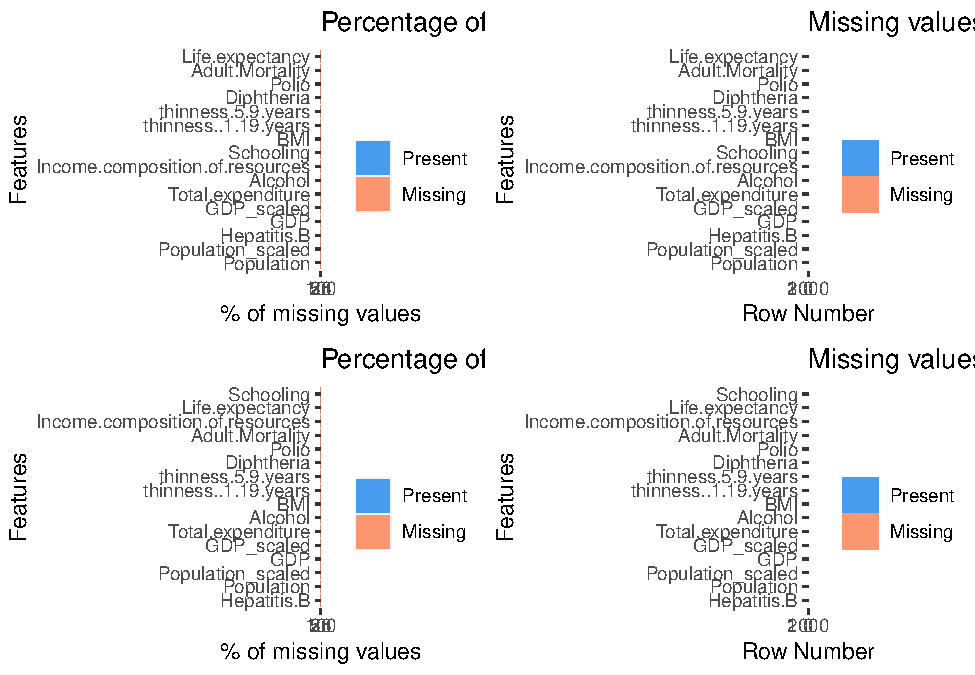
\includegraphics{583Project_files/figure-latex/unnamed-chunk-8-1.pdf}

\begin{Shaded}
\begin{Highlighting}[]
\NormalTok{gridExtra}\SpecialCharTok{::}\FunctionTok{grid.arrange}\NormalTok{(null\_percentage\_dropped.plot, null\_inrow\_dropped.plot, }\AttributeTok{ncol =} \DecValTok{1}\NormalTok{)}
\end{Highlighting}
\end{Shaded}

\begin{verbatim}
## Warning: Removed 8 rows containing missing values (`position_stack()`).
\end{verbatim}

\begin{verbatim}
## Warning: Removed 22224 rows containing missing values (`geom_raster()`).
\end{verbatim}

\includegraphics{583Project_files/figure-latex/unnamed-chunk-8-2.pdf}

There are 2938 no. of rows in the dataset. Acording to our Visualization
on left, there seems to be a correlation in the appearance in missing
data in our orginal data's feature ``population'', ``gdp'' ,
``income.composition.of.resources'' and ``schooling''. We could deal
with this correlation in missing data by removing the the record that
have missing value in all of the listed variables.

\#Check how much records do each country have:

\begin{Shaded}
\begin{Highlighting}[]
\NormalTok{le }\SpecialCharTok{\%\textgreater{}\%} \FunctionTok{group\_by}\NormalTok{(Country) }\SpecialCharTok{\%\textgreater{}\%} \FunctionTok{summarise}\NormalTok{(}\AttributeTok{COUNT =} \FunctionTok{n}\NormalTok{())}
\end{Highlighting}
\end{Shaded}

\begin{verbatim}
## # A tibble: 193 x 2
##    Country             COUNT
##    <chr>               <int>
##  1 Afghanistan            16
##  2 Albania                16
##  3 Algeria                16
##  4 Angola                 16
##  5 Antigua and Barbuda    16
##  6 Argentina              16
##  7 Armenia                16
##  8 Australia              16
##  9 Austria                16
## 10 Azerbaijan             16
## # ... with 183 more rows
\end{verbatim}

\begin{Shaded}
\begin{Highlighting}[]
\NormalTok{le\_dropped }\SpecialCharTok{\%\textgreater{}\%} \FunctionTok{group\_by}\NormalTok{(Country) }\SpecialCharTok{\%\textgreater{}\%} \FunctionTok{summarise}\NormalTok{(}\AttributeTok{COUNT =} \FunctionTok{n}\NormalTok{()) }\CommentTok{\#12 country were removed after dropping some common null value (193{-}181)}
\end{Highlighting}
\end{Shaded}

\begin{verbatim}
## # A tibble: 181 x 2
##    Country             COUNT
##    <chr>               <int>
##  1 Afghanistan            16
##  2 Albania                16
##  3 Algeria                16
##  4 Angola                 16
##  5 Antigua and Barbuda    16
##  6 Argentina              16
##  7 Armenia                16
##  8 Australia              16
##  9 Austria                16
## 10 Azerbaijan             16
## # ... with 171 more rows
\end{verbatim}

\begin{Shaded}
\begin{Highlighting}[]
\CommentTok{\#might need to consider not using this variable }
\end{Highlighting}
\end{Shaded}

\#\#\#\#\#\#\#\#Since we have a better approach, we might need to remove
this\#\#\#\#\#\#\#\#\#\#\#\# Let's set the threshold of 20\% as the max.
proportion of null column to be allowed in a data column. That means,
columns with na over 20\% will be dropped. The threshold is then 587.6.
So, the following `Population' column will be dropped.
\_\_\_\_\_\_\_\_\_\_\_\_\_\_\_\_\_\_\_\_\_\_\_\_\_\_\_\_\_\_\_\_\_\_\_\_\_\_\_\_\_\_\_\_\_\_\_\_\_\_\_\_

\#head(le) le \textless- subset(le,select=-c(Population)) \# also
Population\_Scaled le \textless-
subset(le,select=-c(Population\_scaled))

\begin{center}\rule{0.5\linewidth}{0.5pt}\end{center}

For the other values, we will set the na to the respective column mean
for the subsequent analysis.

\begin{Shaded}
\begin{Highlighting}[]
\ControlFlowTok{for}\NormalTok{(i }\ControlFlowTok{in} \DecValTok{1}\SpecialCharTok{:}\FunctionTok{ncol}\NormalTok{(le\_dropped)) \{                                   }\CommentTok{\# Replace NA in all columns}
\NormalTok{  le\_dropped[ , i][}\FunctionTok{is.na}\NormalTok{(le\_dropped[ , i])] }\OtherTok{\textless{}{-}} \FunctionTok{mean}\NormalTok{(le\_dropped[ , i], }\AttributeTok{na.rm =} \ConstantTok{TRUE}\NormalTok{)}
\NormalTok{\}}
\end{Highlighting}
\end{Shaded}

Now, all na have been handled! Let's continue our analysis.

\hypertarget{overall-general-life-expectancy-trend}{%
\subsubsection{Overall General Life Expectancy
Trend}\label{overall-general-life-expectancy-trend}}

Purpose : Do some visualisation to explore and identify the general data
pattern, trends and clusters, etc

\begin{Shaded}
\begin{Highlighting}[]
\FunctionTok{library}\NormalTok{(ggplot2)}
\CommentTok{\#install.packages("tidyverse")}
\FunctionTok{library}\NormalTok{(tidyverse)}

\NormalTok{le\_dropped }\SpecialCharTok{\%\textgreater{}\%}
  \FunctionTok{group\_by}\NormalTok{(Year) }\SpecialCharTok{\%\textgreater{}\%}
  \FunctionTok{summarise}\NormalTok{(}\AttributeTok{Life.expectancy =} \FunctionTok{mean}\NormalTok{(Life.expectancy)) }\SpecialCharTok{\%\textgreater{}\%}
  \FunctionTok{ggplot}\NormalTok{(}\FunctionTok{aes}\NormalTok{(}\AttributeTok{x=}\NormalTok{Year,}
             \AttributeTok{y=}\NormalTok{Life.expectancy)) }\SpecialCharTok{+}    
  \FunctionTok{geom\_line}\NormalTok{()}
\end{Highlighting}
\end{Shaded}

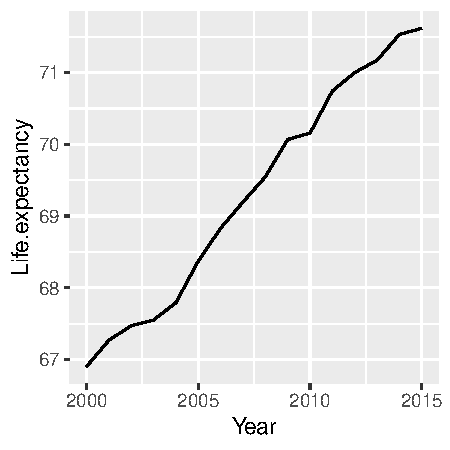
\includegraphics{583Project_files/figure-latex/unnamed-chunk-11-1.pdf}

Findings :

\begin{itemize}
\tightlist
\item
  The general life expectancy has been steadily increasing duration the
  year
\item
  Average Life expectancy increase from about 67 to 71.5 in 15 years.
\end{itemize}

\begin{Shaded}
\begin{Highlighting}[]
\NormalTok{le\_dropped }\SpecialCharTok{\%\textgreater{}\%}
  \FunctionTok{group\_by}\NormalTok{(Status) }\SpecialCharTok{\%\textgreater{}\%}
  \FunctionTok{summarise}\NormalTok{(}\AttributeTok{Life.expectancy =} \FunctionTok{mean}\NormalTok{(Life.expectancy)) }\SpecialCharTok{\%\textgreater{}\%}
  \FunctionTok{ggplot}\NormalTok{(}\FunctionTok{aes}\NormalTok{(}\AttributeTok{x=}\NormalTok{Status,}
             \AttributeTok{y=}\NormalTok{Life.expectancy,}
             \AttributeTok{fill=}\NormalTok{Status)) }\SpecialCharTok{+}    
  \FunctionTok{geom\_bar}\NormalTok{(}\AttributeTok{stat =} \StringTok{"identity"}\NormalTok{)}\SpecialCharTok{+} \FunctionTok{scale\_fill\_manual}\NormalTok{(}\AttributeTok{values=}\FunctionTok{c}\NormalTok{(}\StringTok{\textquotesingle{}dodgerblue2\textquotesingle{}}\NormalTok{, }\StringTok{\textquotesingle{}coral\textquotesingle{}}\NormalTok{))}
\end{Highlighting}
\end{Shaded}

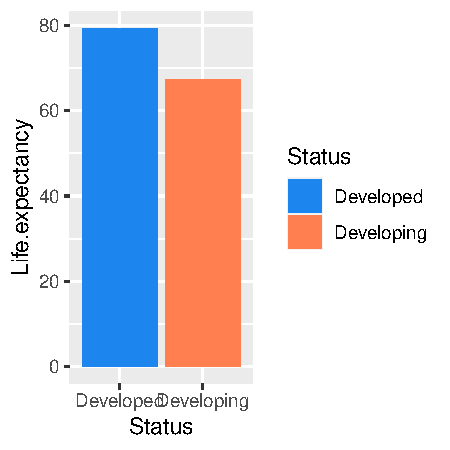
\includegraphics{583Project_files/figure-latex/unnamed-chunk-12-1.pdf}

Finding :

\begin{itemize}
\tightlist
\item
  Life expectancy of Developed countries are significantly higher than
  that of Developing countries.
\end{itemize}

\begin{Shaded}
\begin{Highlighting}[]
\NormalTok{le\_dropped.pivot }\OtherTok{\textless{}{-}} \FunctionTok{pivot\_longer}\NormalTok{(le\_dropped,}\FunctionTok{c}\NormalTok{(Adult.Mortality,under.five.deaths,infant.deaths),}\AttributeTok{names\_to=}\StringTok{\textquotesingle{}Mortality.Group\textquotesingle{}}\NormalTok{,}\AttributeTok{values\_to=}\StringTok{\textquotesingle{}Mortality.Rate\textquotesingle{}}\NormalTok{)}
\FunctionTok{require}\NormalTok{(gridExtra)}

\NormalTok{le\_dropped.pivot.area }\OtherTok{\textless{}{-}}\NormalTok{ le\_dropped.pivot }\SpecialCharTok{\%\textgreater{}\%}
  \FunctionTok{group\_by}\NormalTok{(Year,Mortality.Group) }\SpecialCharTok{\%\textgreater{}\%}
  \FunctionTok{summarise}\NormalTok{(}\AttributeTok{Mortality.Rate =} \FunctionTok{mean}\NormalTok{(Mortality.Rate)) }\SpecialCharTok{\%\textgreater{}\%}
  \FunctionTok{ggplot}\NormalTok{(}\FunctionTok{aes}\NormalTok{(}\AttributeTok{x=}\NormalTok{Year,}
             \AttributeTok{y=}\NormalTok{Mortality.Rate,}
             \AttributeTok{fill=}\NormalTok{Mortality.Group)) }\SpecialCharTok{+}
  \FunctionTok{geom\_area}\NormalTok{(}\AttributeTok{position=}\StringTok{"stack"}\NormalTok{,}\AttributeTok{stat=}\StringTok{"identity"}\NormalTok{)}

\NormalTok{le\_dropped.pivot.line }\OtherTok{\textless{}{-}}\NormalTok{ le\_dropped.pivot }\SpecialCharTok{\%\textgreater{}\%}
  \FunctionTok{group\_by}\NormalTok{(Year,Mortality.Group) }\SpecialCharTok{\%\textgreater{}\%}
  \FunctionTok{summarise}\NormalTok{(}\AttributeTok{Mortality.Rate =} \FunctionTok{mean}\NormalTok{(Mortality.Rate)) }\SpecialCharTok{\%\textgreater{}\%}
  \FunctionTok{ggplot}\NormalTok{(}\FunctionTok{aes}\NormalTok{(}\AttributeTok{x=}\NormalTok{Year,}
             \AttributeTok{y=}\NormalTok{Mortality.Rate,}
             \AttributeTok{color=}\NormalTok{Mortality.Group)) }\SpecialCharTok{+}
  \FunctionTok{geom\_line}\NormalTok{()}

\FunctionTok{grid.arrange}\NormalTok{(le\_dropped.pivot.area,le\_dropped.pivot.line, }\AttributeTok{ncol=}\DecValTok{2}\NormalTok{)}
\end{Highlighting}
\end{Shaded}

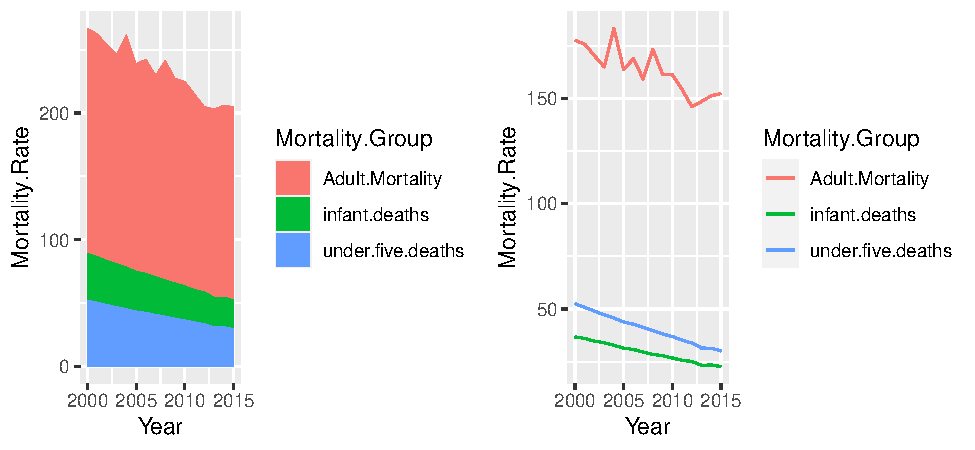
\includegraphics{583Project_files/figure-latex/unnamed-chunk-13-1.pdf}

Findings :

\begin{itemize}
\tightlist
\item
  The mortality rate of all three age groups are generally decreasing as
  a whole
\item
  The mortality rate of the adult group, however, have fluctuation
  within the period
\end{itemize}

\#\#\#\#\#\#\#\#\#\#\#\#\#\#\#\#\#\#\#\#\#\#Variable Selections (BIC
backwards):\#\#\#\#\#\#\#\#\#\#\#\#\#\#\#\#\#\#\#\#\#
\#\#\#\#\#\#\#\#\#\#\#\#\#\#\#\#\#\#\#\#\#\#\#\#\#\#\#\#\#\#\#\#\#\#\#\#\#\#\#\#\#\#\#\#\#\#\#\#\#\#\#\#\#\#\#\#\#\#\#\#\#\#\#\#\#\#\#\#\#\#\#\#\#\#\#\#\#\#\#

\begin{Shaded}
\begin{Highlighting}[]
\FunctionTok{head}\NormalTok{(le\_dropped)}
\end{Highlighting}
\end{Shaded}

\begin{verbatim}
##       Country Year     Status Life.expectancy Adult.Mortality infant.deaths
## 1 Afghanistan 2015 Developing            65.0             263            62
## 2 Afghanistan 2014 Developing            59.9             271            64
## 3 Afghanistan 2013 Developing            59.9             268            66
## 4 Afghanistan 2012 Developing            59.5             272            69
## 5 Afghanistan 2011 Developing            59.2             275            71
## 6 Afghanistan 2010 Developing            58.8             279            74
##   Alcohol Hepatitis.B Measles  BMI under.five.deaths Polio Total.expenditure
## 1    0.01          65    1154 19.1                83     6              8.16
## 2    0.01          62     492 18.6                86    58              8.18
## 3    0.01          64     430 18.1                89    62              8.13
## 4    0.01          67    2787 17.6                93    67              8.52
## 5    0.01          68    3013 17.2                97    68              7.87
## 6    0.01          66    1989 16.7               102    66              9.20
##   Diphtheria HIV.AIDS       GDP Population thinness..1.19.years
## 1         65      0.1 584.25921   33736494                 17.2
## 2         62      0.1 612.69651     327582                 17.5
## 3         64      0.1 631.74498   31731688                 17.7
## 4         67      0.1 669.95900    3696958                 17.9
## 5         68      0.1  63.53723    2978599                 18.2
## 6         66      0.1 553.32894    2883167                 18.4
##   thinness.5.9.years Income.composition.of.resources Schooling Status.val
## 1               17.3                           0.479      10.1          0
## 2               17.5                           0.476      10.0          0
## 3               17.7                           0.470       9.9          0
## 4               18.0                           0.463       9.8          0
## 5               18.2                           0.454       9.5          0
## 6               18.4                           0.448       9.2          0
##   GDP_scaled Population_scaled
## 1 -0.4834490         0.3439174
## 2 -0.4814562        -0.2036611
## 3 -0.4801214         0.3110582
## 4 -0.4774435        -0.1484364
## 5 -0.5199393        -0.1602105
## 6 -0.4856165        -0.1617746
\end{verbatim}

\begin{Shaded}
\begin{Highlighting}[]
\CommentTok{\#droped GDP,Population}
\NormalTok{df }\OtherTok{=} \FunctionTok{subset}\NormalTok{(le\_dropped, }\AttributeTok{select =} \SpecialCharTok{{-}}\FunctionTok{c}\NormalTok{(Country,GDP,Population) )}
\CommentTok{\#droped GDP\_scaled,Population\_scaled}
\NormalTok{df\_ns }\OtherTok{=} \FunctionTok{subset}\NormalTok{(le\_dropped, }\AttributeTok{select =}\SpecialCharTok{{-}}\FunctionTok{c}\NormalTok{(Country,GDP\_scaled,Population\_scaled) )}
\FunctionTok{head}\NormalTok{(df)}
\end{Highlighting}
\end{Shaded}

\begin{verbatim}
##   Year     Status Life.expectancy Adult.Mortality infant.deaths Alcohol
## 1 2015 Developing            65.0             263            62    0.01
## 2 2014 Developing            59.9             271            64    0.01
## 3 2013 Developing            59.9             268            66    0.01
## 4 2012 Developing            59.5             272            69    0.01
## 5 2011 Developing            59.2             275            71    0.01
## 6 2010 Developing            58.8             279            74    0.01
##   Hepatitis.B Measles  BMI under.five.deaths Polio Total.expenditure Diphtheria
## 1          65    1154 19.1                83     6              8.16         65
## 2          62     492 18.6                86    58              8.18         62
## 3          64     430 18.1                89    62              8.13         64
## 4          67    2787 17.6                93    67              8.52         67
## 5          68    3013 17.2                97    68              7.87         68
## 6          66    1989 16.7               102    66              9.20         66
##   HIV.AIDS thinness..1.19.years thinness.5.9.years
## 1      0.1                 17.2               17.3
## 2      0.1                 17.5               17.5
## 3      0.1                 17.7               17.7
## 4      0.1                 17.9               18.0
## 5      0.1                 18.2               18.2
## 6      0.1                 18.4               18.4
##   Income.composition.of.resources Schooling Status.val GDP_scaled
## 1                           0.479      10.1          0 -0.4834490
## 2                           0.476      10.0          0 -0.4814562
## 3                           0.470       9.9          0 -0.4801214
## 4                           0.463       9.8          0 -0.4774435
## 5                           0.454       9.5          0 -0.5199393
## 6                           0.448       9.2          0 -0.4856165
##   Population_scaled
## 1         0.3439174
## 2        -0.2036611
## 3         0.3110582
## 4        -0.1484364
## 5        -0.1602105
## 6        -0.1617746
\end{verbatim}

Let's look at the distribution of different columns in the dataset.

\begin{Shaded}
\begin{Highlighting}[]
\CommentTok{\#install.packages("Hmisc")}
\CommentTok{\#library(ggplot2)}
\CommentTok{\#library(tidyr)}
\CommentTok{\#hist.data.frame(df)}
\end{Highlighting}
\end{Shaded}

As we see, the response variable Life Expectancy is normally distributed
and so our first try is to see if MLR is able to predict well. Also,
using this model and running a BIC on it, we can understand the columns
that are important.

\begin{Shaded}
\begin{Highlighting}[]
\NormalTok{lmmod }\OtherTok{\textless{}{-}} \FunctionTok{lm}\NormalTok{(Life.expectancy}\SpecialCharTok{\textasciitilde{}}\NormalTok{., }\AttributeTok{data =}\NormalTok{ df)}
\FunctionTok{summary}\NormalTok{(lmmod)}
\end{Highlighting}
\end{Shaded}

\begin{verbatim}
## 
## Call:
## lm(formula = Life.expectancy ~ ., data = df)
## 
## Residuals:
##      Min       1Q   Median       3Q      Max 
## -21.6365  -2.1904  -0.0813   2.2726  18.6972 
## 
## Coefficients: (1 not defined because of singularities)
##                                   Estimate Std. Error t value Pr(>|t|)    
## (Intercept)                      1.366e+02  3.413e+01   4.003 6.41e-05 ***
## Year                            -4.046e-02  1.707e-02  -2.369 0.017888 *  
## StatusDeveloping                -1.340e+00  2.679e-01  -5.002 6.02e-07 ***
## Adult.Mortality                 -1.674e-02  7.966e-04 -21.011  < 2e-16 ***
## infant.deaths                    9.138e-02  8.101e-03  11.280  < 2e-16 ***
## Alcohol                         -2.433e-02  2.584e-02  -0.941 0.346621    
## Hepatitis.B                     -1.387e-02  3.833e-03  -3.617 0.000303 ***
## Measles                         -9.298e-06  8.300e-06  -1.120 0.262740    
## BMI                              3.946e-02  4.887e-03   8.074 1.01e-15 ***
## under.five.deaths               -6.807e-02  5.944e-03 -11.453  < 2e-16 ***
## Polio                            2.489e-02  4.482e-03   5.554 3.06e-08 ***
## Total.expenditure                5.942e-02  3.421e-02   1.737 0.082527 .  
## Diphtheria                       3.343e-02  4.749e-03   7.040 2.41e-12 ***
## HIV.AIDS                        -4.878e-01  1.705e-02 -28.609  < 2e-16 ***
## thinness..1.19.years            -7.134e-02  4.860e-02  -1.468 0.142241    
## thinness.5.9.years               6.001e-03  4.793e-02   0.125 0.900374    
## Income.composition.of.resources  6.736e+00  6.152e-01  10.949  < 2e-16 ***
## Schooling                        7.798e-01  4.083e-02  19.097  < 2e-16 ***
## Status.val                              NA         NA      NA       NA    
## GDP_scaled                       7.523e-01  9.195e-02   8.182 4.23e-16 ***
## Population_scaled               -6.306e-02  9.873e-02  -0.639 0.523086    
## ---
## Signif. codes:  0 '***' 0.001 '**' 0.01 '*' 0.05 '.' 0.1 ' ' 1
## 
## Residual standard error: 3.86 on 2758 degrees of freedom
## Multiple R-squared:  0.831,  Adjusted R-squared:  0.8299 
## F-statistic: 713.8 on 19 and 2758 DF,  p-value: < 2.2e-16
\end{verbatim}

\begin{Shaded}
\begin{Highlighting}[]
\FunctionTok{plot}\NormalTok{(lmmod)}
\end{Highlighting}
\end{Shaded}

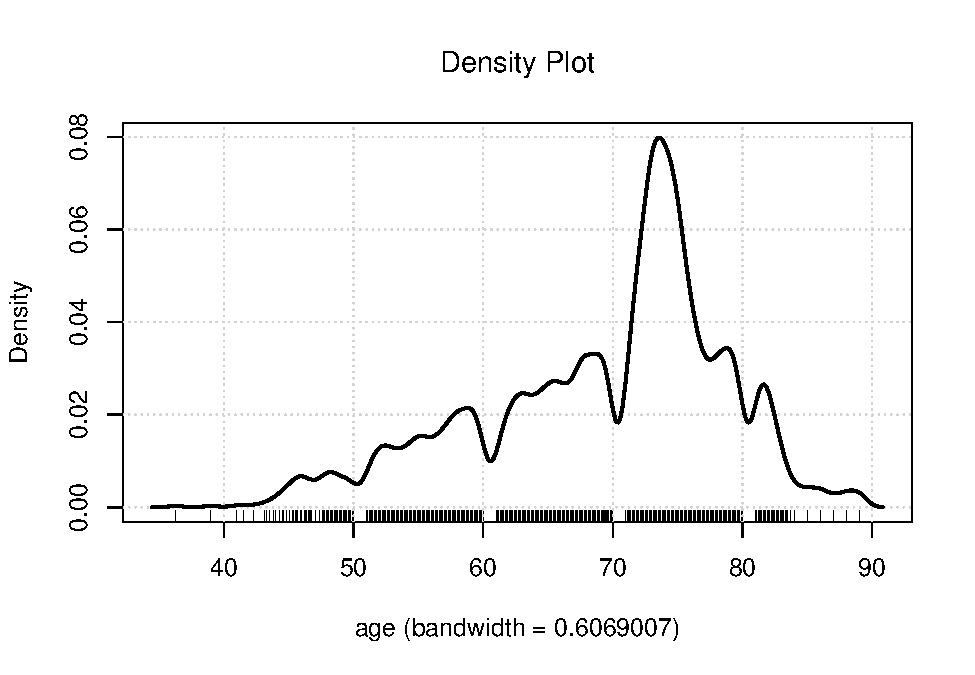
\includegraphics{583Project_files/figure-latex/unnamed-chunk-18-1.pdf}
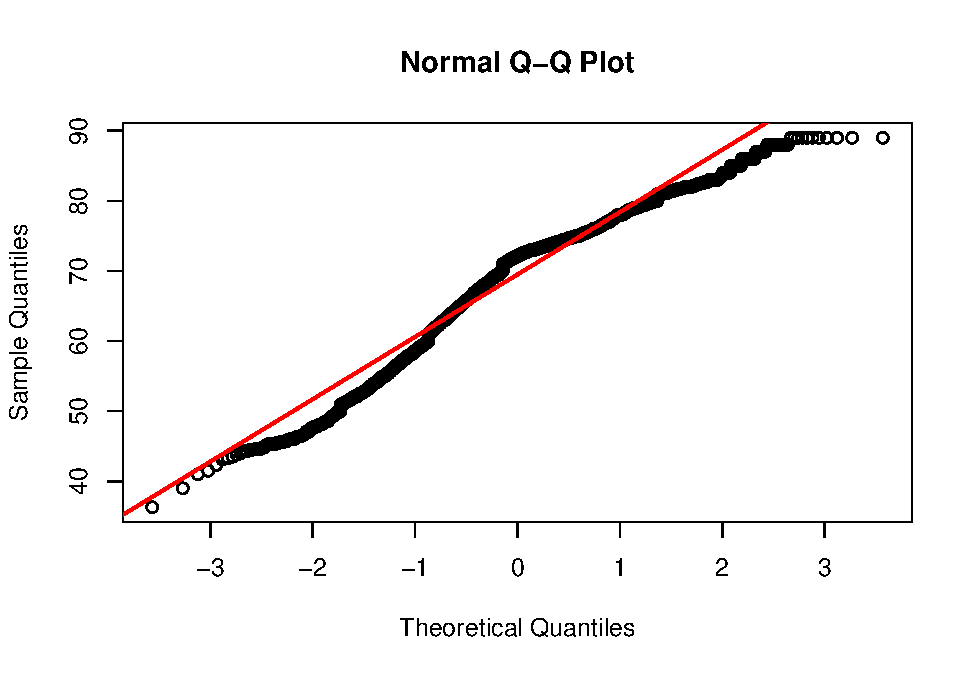
\includegraphics{583Project_files/figure-latex/unnamed-chunk-18-2.pdf}
\includegraphics{583Project_files/figure-latex/unnamed-chunk-18-3.pdf}
\includegraphics{583Project_files/figure-latex/unnamed-chunk-18-4.pdf}

\begin{Shaded}
\begin{Highlighting}[]
\NormalTok{model.step.bic }\OtherTok{\textless{}{-}} \FunctionTok{step}\NormalTok{(lmmod,}\AttributeTok{k=}\FunctionTok{log}\NormalTok{(}\FunctionTok{nrow}\NormalTok{(df)))}
\end{Highlighting}
\end{Shaded}

\begin{verbatim}
## Start:  AIC=7642.14
## Life.expectancy ~ Year + Status + Adult.Mortality + infant.deaths + 
##     Alcohol + Hepatitis.B + Measles + BMI + under.five.deaths + 
##     Polio + Total.expenditure + Diphtheria + HIV.AIDS + thinness..1.19.years + 
##     thinness.5.9.years + Income.composition.of.resources + Schooling + 
##     Status.val + GDP_scaled + Population_scaled
## 
## 
## Step:  AIC=7642.14
## Life.expectancy ~ Year + Status + Adult.Mortality + infant.deaths + 
##     Alcohol + Hepatitis.B + Measles + BMI + under.five.deaths + 
##     Polio + Total.expenditure + Diphtheria + HIV.AIDS + thinness..1.19.years + 
##     thinness.5.9.years + Income.composition.of.resources + Schooling + 
##     GDP_scaled + Population_scaled
## 
##                                   Df Sum of Sq   RSS    AIC
## - thinness.5.9.years               1       0.2 41083 7634.2
## - Population_scaled                1       6.1 41089 7634.6
## - Alcohol                          1      13.2 41096 7635.1
## - Measles                          1      18.7 41102 7635.5
## - thinness..1.19.years             1      32.1 41115 7636.4
## - Total.expenditure                1      44.9 41128 7637.3
## - Year                             1      83.6 41167 7639.9
## <none>                                         41083 7642.1
## - Hepatitis.B                      1     194.9 41278 7647.4
## - Status                           1     372.7 41456 7659.3
## - Polio                            1     459.5 41543 7665.1
## - Diphtheria                       1     738.4 41821 7683.7
## - BMI                              1     971.0 42054 7699.1
## - GDP_scaled                       1     997.1 42080 7700.8
## - Income.composition.of.resources  1    1785.7 42869 7752.4
## - infant.deaths                    1    1895.3 42978 7759.5
## - under.five.deaths                1    1953.9 43037 7763.3
## - Schooling                        1    5432.2 46515 7979.2
## - Adult.Mortality                  1    6575.9 47659 8046.7
## - HIV.AIDS                         1   12191.8 53275 8356.1
## 
## Step:  AIC=7634.23
## Life.expectancy ~ Year + Status + Adult.Mortality + infant.deaths + 
##     Alcohol + Hepatitis.B + Measles + BMI + under.five.deaths + 
##     Polio + Total.expenditure + Diphtheria + HIV.AIDS + thinness..1.19.years + 
##     Income.composition.of.resources + Schooling + GDP_scaled + 
##     Population_scaled
## 
##                                   Df Sum of Sq   RSS    AIC
## - Population_scaled                1       6.1 41089 7626.7
## - Alcohol                          1      13.2 41097 7627.2
## - Measles                          1      18.8 41102 7627.6
## - Total.expenditure                1      44.7 41128 7629.3
## - Year                             1      83.7 41167 7632.0
## <none>                                         41083 7634.2
## - thinness..1.19.years             1     121.3 41205 7634.5
## - Hepatitis.B                      1     195.0 41278 7639.5
## - Status                           1     372.5 41456 7651.4
## - Polio                            1     459.3 41543 7657.2
## - Diphtheria                       1     739.0 41822 7675.8
## - BMI                              1     982.6 42066 7692.0
## - GDP_scaled                       1     997.0 42080 7692.9
## - Income.composition.of.resources  1    1786.4 42870 7744.5
## - infant.deaths                    1    1904.2 42988 7752.2
## - under.five.deaths                1    1959.8 43043 7755.8
## - Schooling                        1    5435.3 46519 7971.5
## - Adult.Mortality                  1    6580.5 47664 8039.0
## - HIV.AIDS                         1   12195.3 53279 8348.4
## 
## Step:  AIC=7626.72
## Life.expectancy ~ Year + Status + Adult.Mortality + infant.deaths + 
##     Alcohol + Hepatitis.B + Measles + BMI + under.five.deaths + 
##     Polio + Total.expenditure + Diphtheria + HIV.AIDS + thinness..1.19.years + 
##     Income.composition.of.resources + Schooling + GDP_scaled
## 
##                                   Df Sum of Sq   RSS    AIC
## - Alcohol                          1      13.6 41103 7619.7
## - Measles                          1      18.6 41108 7620.0
## - Total.expenditure                1      45.5 41135 7621.9
## - Year                             1      84.8 41174 7624.5
## <none>                                         41089 7626.7
## - thinness..1.19.years             1     122.4 41212 7627.1
## - Hepatitis.B                      1     191.6 41281 7631.7
## - Status                           1     374.7 41464 7644.0
## - Polio                            1     458.7 41548 7649.6
## - Diphtheria                       1     735.5 41825 7668.1
## - BMI                              1     979.4 42069 7684.2
## - GDP_scaled                       1     995.6 42085 7685.3
## - Income.composition.of.resources  1    1787.5 42877 7737.1
## - infant.deaths                    1    1925.1 43015 7746.0
## - under.five.deaths                1    1962.6 43052 7748.4
## - Schooling                        1    5429.2 46519 7963.5
## - Adult.Mortality                  1    6579.8 47669 8031.4
## - HIV.AIDS                         1   12192.1 53282 8340.6
## 
## Step:  AIC=7619.71
## Life.expectancy ~ Year + Status + Adult.Mortality + infant.deaths + 
##     Hepatitis.B + Measles + BMI + under.five.deaths + Polio + 
##     Total.expenditure + Diphtheria + HIV.AIDS + thinness..1.19.years + 
##     Income.composition.of.resources + Schooling + GDP_scaled
## 
##                                   Df Sum of Sq   RSS    AIC
## - Measles                          1      19.9 41123 7613.1
## - Total.expenditure                1      40.2 41143 7614.5
## - Year                             1      76.6 41180 7617.0
## - thinness..1.19.years             1     112.0 41215 7619.3
## <none>                                         41103 7619.7
## - Hepatitis.B                      1     189.4 41292 7624.6
## - Status                           1     370.3 41473 7636.7
## - Polio                            1     459.4 41562 7642.7
## - Diphtheria                       1     730.0 41833 7660.7
## - BMI                              1     981.5 42084 7677.3
## - GDP_scaled                       1     990.9 42094 7678.0
## - Income.composition.of.resources  1    1778.4 42881 7729.4
## - infant.deaths                    1    1999.0 43102 7743.7
## - under.five.deaths                1    2043.5 43147 7746.6
## - Schooling                        1    5595.5 46699 7966.3
## - Adult.Mortality                  1    6738.3 47841 8033.5
## - HIV.AIDS                         1   12244.2 53347 8336.1
## 
## Step:  AIC=7613.12
## Life.expectancy ~ Year + Status + Adult.Mortality + infant.deaths + 
##     Hepatitis.B + BMI + under.five.deaths + Polio + Total.expenditure + 
##     Diphtheria + HIV.AIDS + thinness..1.19.years + Income.composition.of.resources + 
##     Schooling + GDP_scaled
## 
##                                   Df Sum of Sq   RSS    AIC
## - Total.expenditure                1      41.5 41164 7608.0
## - Year                             1      72.0 41195 7610.1
## - thinness..1.19.years             1     107.6 41230 7612.4
## <none>                                         41123 7613.1
## - Hepatitis.B                      1     192.2 41315 7618.1
## - Status                           1     373.5 41496 7630.3
## - Polio                            1     461.4 41584 7636.2
## - Diphtheria                       1     729.9 41853 7654.1
## - GDP_scaled                       1     992.5 42115 7671.4
## - BMI                              1    1003.5 42126 7672.2
## - Income.composition.of.resources  1    1790.9 42914 7723.6
## - infant.deaths                    1    2035.8 43159 7739.4
## - under.five.deaths                1    2120.0 43243 7744.8
## - Schooling                        1    5585.1 46708 7959.0
## - Adult.Mortality                  1    6723.0 47846 8025.8
## - HIV.AIDS                         1   12287.1 53410 8331.5
## 
## Step:  AIC=7607.99
## Life.expectancy ~ Year + Status + Adult.Mortality + infant.deaths + 
##     Hepatitis.B + BMI + under.five.deaths + Polio + Diphtheria + 
##     HIV.AIDS + thinness..1.19.years + Income.composition.of.resources + 
##     Schooling + GDP_scaled
## 
##                                   Df Sum of Sq   RSS    AIC
## - Year                             1      63.4 41228 7604.3
## <none>                                         41164 7608.0
## - thinness..1.19.years             1     125.4 41290 7608.5
## - Hepatitis.B                      1     197.5 41362 7613.4
## - Status                           1     423.2 41588 7628.5
## - Polio                            1     466.7 41631 7631.4
## - Diphtheria                       1     745.6 41910 7649.9
## - GDP_scaled                       1     985.0 42149 7665.8
## - BMI                              1    1039.6 42204 7669.3
## - Income.composition.of.resources  1    1756.0 42920 7716.1
## - infant.deaths                    1    2030.0 43194 7733.8
## - under.five.deaths                1    2114.2 43279 7739.2
## - Schooling                        1    5689.0 46853 7959.7
## - Adult.Mortality                  1    6730.8 47895 8020.8
## - HIV.AIDS                         1   12261.5 53426 8324.3
## 
## Step:  AIC=7604.34
## Life.expectancy ~ Status + Adult.Mortality + infant.deaths + 
##     Hepatitis.B + BMI + under.five.deaths + Polio + Diphtheria + 
##     HIV.AIDS + thinness..1.19.years + Income.composition.of.resources + 
##     Schooling + GDP_scaled
## 
##                                   Df Sum of Sq   RSS    AIC
## <none>                                         41228 7604.3
## - thinness..1.19.years             1     136.4 41364 7605.6
## - Hepatitis.B                      1     207.5 41435 7610.4
## - Status                           1     480.3 41708 7628.6
## - Polio                            1     486.6 41714 7629.0
## - Diphtheria                       1     728.9 41957 7645.1
## - GDP_scaled                       1     967.2 42195 7660.8
## - BMI                              1    1045.1 42273 7665.9
## - Income.composition.of.resources  1    1695.9 42924 7708.4
## - infant.deaths                    1    2044.7 43272 7730.9
## - under.five.deaths                1    2127.7 43355 7736.2
## - Schooling                        1    5629.3 46857 7952.0
## - Adult.Mortality                  1    6901.0 48129 8026.4
## - HIV.AIDS                         1   12231.6 53459 8318.2
\end{verbatim}

\begin{Shaded}
\begin{Highlighting}[]
\FunctionTok{summary}\NormalTok{(model.step.bic)}
\end{Highlighting}
\end{Shaded}

\begin{verbatim}
## 
## Call:
## lm(formula = Life.expectancy ~ Status + Adult.Mortality + infant.deaths + 
##     Hepatitis.B + BMI + under.five.deaths + Polio + Diphtheria + 
##     HIV.AIDS + thinness..1.19.years + Income.composition.of.resources + 
##     Schooling + GDP_scaled, data = df)
## 
## Residuals:
##      Min       1Q   Median       3Q      Max 
## -21.1806  -2.1862  -0.1082   2.2527  18.3932 
## 
## Coefficients:
##                                   Estimate Std. Error t value Pr(>|t|)    
## (Intercept)                     56.0248606  0.6068087  92.327  < 2e-16 ***
## StatusDeveloping                -1.3992281  0.2465832  -5.674 1.54e-08 ***
## Adult.Mortality                 -0.0169017  0.0007858 -21.509  < 2e-16 ***
## infant.deaths                    0.0923034  0.0078837  11.708  < 2e-16 ***
## Hepatitis.B                     -0.0142558  0.0038221  -3.730 0.000195 ***
## BMI                              0.0404056  0.0048271   8.371  < 2e-16 ***
## under.five.deaths               -0.0692931  0.0058018 -11.943  < 2e-16 ***
## Polio                            0.0255695  0.0044766   5.712 1.24e-08 ***
## Diphtheria                       0.0331225  0.0047383   6.990 3.42e-12 ***
## HIV.AIDS                        -0.4819251  0.0168292 -28.636  < 2e-16 ***
## thinness..1.19.years            -0.0682138  0.0225535  -3.025 0.002513 ** 
## Income.composition.of.resources  6.4576087  0.6056113  10.663  < 2e-16 ***
## Schooling                        0.7678056  0.0395229  19.427  < 2e-16 ***
## GDP_scaled                       0.7397976  0.0918701   8.053 1.19e-15 ***
## ---
## Signif. codes:  0 '***' 0.001 '**' 0.01 '*' 0.05 '.' 0.1 ' ' 1
## 
## Residual standard error: 3.862 on 2764 degrees of freedom
## Multiple R-squared:  0.8304, Adjusted R-squared:  0.8296 
## F-statistic:  1041 on 13 and 2764 DF,  p-value: < 2.2e-16
\end{verbatim}

try clustering to understand grouping in data so we can separate may be
developing vs developed countries

From below results, we do not see any such cluster to split.

\begin{Shaded}
\begin{Highlighting}[]
\FunctionTok{library}\NormalTok{(mclust)}
\end{Highlighting}
\end{Shaded}

\begin{verbatim}
## Warning: package 'mclust' was built under R version 4.2.2
\end{verbatim}

\begin{verbatim}
## Package 'mclust' version 6.0.0
## Type 'citation("mclust")' for citing this R package in publications.
\end{verbatim}

\begin{verbatim}
## 
## Attaching package: 'mclust'
\end{verbatim}

\begin{verbatim}
## The following object is masked from 'package:purrr':
## 
##     map
\end{verbatim}

\begin{Shaded}
\begin{Highlighting}[]
\NormalTok{clus }\OtherTok{\textless{}{-}} \FunctionTok{Mclust}\NormalTok{(df)}
\FunctionTok{summary}\NormalTok{(clus)}
\end{Highlighting}
\end{Shaded}

\begin{verbatim}
## ---------------------------------------------------- 
## Gaussian finite mixture model fitted by EM algorithm 
## ---------------------------------------------------- 
## 
## Mclust XXX (ellipsoidal multivariate normal) model with 1 component: 
## 
##  log-likelihood    n  df       BIC       ICL
##       -101559.5 2778 252 -205117.2 -205117.2
## 
## Clustering table:
##    1 
## 2778
\end{verbatim}

\begin{Shaded}
\begin{Highlighting}[]
\CommentTok{\#No clusters seen in original dataset}
\end{Highlighting}
\end{Shaded}

Variable selection using BIC and VIF, VIF also increases model
performance:

\begin{Shaded}
\begin{Highlighting}[]
\FunctionTok{library}\NormalTok{(car)}
\end{Highlighting}
\end{Shaded}

\begin{verbatim}
## Warning: package 'car' was built under R version 4.2.2
\end{verbatim}

\begin{verbatim}
## Loading required package: carData
\end{verbatim}

\begin{verbatim}
## Warning: package 'carData' was built under R version 4.2.2
\end{verbatim}

\begin{verbatim}
## 
## Attaching package: 'car'
\end{verbatim}

\begin{verbatim}
## The following object is masked from 'package:purrr':
## 
##     some
\end{verbatim}

\begin{verbatim}
## The following object is masked from 'package:dplyr':
## 
##     recode
\end{verbatim}

\begin{Shaded}
\begin{Highlighting}[]
\FunctionTok{vif}\NormalTok{(model.step.bic)}
\end{Highlighting}
\end{Shaded}

\begin{verbatim}
##                          Status                 Adult.Mortality 
##                        1.575522                        1.734550 
##                   infant.deaths                     Hepatitis.B 
##                      166.764248                        1.392762 
##                             BMI               under.five.deaths 
##                        1.700393                      166.967503 
##                           Polio                      Diphtheria 
##                        1.985023                        2.246470 
##                        HIV.AIDS            thinness..1.19.years 
##                        1.414455                        1.875037 
## Income.composition.of.resources                       Schooling 
##                        3.029591                        3.277562 
##                      GDP_scaled 
##                        1.408386
\end{verbatim}

\begin{Shaded}
\begin{Highlighting}[]
\CommentTok{\#removed one of infant.deaths or under.five.deaths}
\end{Highlighting}
\end{Shaded}

\begin{Shaded}
\begin{Highlighting}[]
\NormalTok{df1}\OtherTok{\textless{}{-}}\NormalTok{df[,}\FunctionTok{c}\NormalTok{(}\StringTok{\textquotesingle{}Life.expectancy\textquotesingle{}}\NormalTok{,}\StringTok{\textquotesingle{}Status\textquotesingle{}}\NormalTok{,}\StringTok{\textquotesingle{}Adult.Mortality\textquotesingle{}}\NormalTok{,}\StringTok{\textquotesingle{}infant.deaths\textquotesingle{}}\NormalTok{,}\StringTok{\textquotesingle{}under.five.deaths\textquotesingle{}}\NormalTok{,}
      \StringTok{\textquotesingle{}Hepatitis.B\textquotesingle{}}\NormalTok{,}\StringTok{\textquotesingle{}BMI\textquotesingle{}}\NormalTok{,}\StringTok{\textquotesingle{}Polio\textquotesingle{}}\NormalTok{,}\StringTok{\textquotesingle{}Diphtheria\textquotesingle{}}\NormalTok{,}
      \StringTok{\textquotesingle{}HIV.AIDS\textquotesingle{}}\NormalTok{,}\StringTok{\textquotesingle{}thinness..1.19.years\textquotesingle{}}\NormalTok{,}\StringTok{\textquotesingle{}Income.composition.of.resources\textquotesingle{}}\NormalTok{,}\StringTok{\textquotesingle{}Schooling\textquotesingle{}}\NormalTok{,}\StringTok{\textquotesingle{}GDP\_scaled\textquotesingle{}}\NormalTok{)]}

\NormalTok{df1}\SpecialCharTok{$}\NormalTok{Status }\OtherTok{\textless{}{-}} \FunctionTok{factor}\NormalTok{(df1}\SpecialCharTok{$}\NormalTok{Status)}
\CommentTok{\#removed \textquotesingle{}under.five.deaths\textquotesingle{}, due to vif {-} multi collinearity from BIC selection but it decreased model}
\CommentTok{\#performance so should we retain it?}
\FunctionTok{head}\NormalTok{(df1)}
\end{Highlighting}
\end{Shaded}

\begin{verbatim}
##   Life.expectancy     Status Adult.Mortality infant.deaths under.five.deaths
## 1            65.0 Developing             263            62                83
## 2            59.9 Developing             271            64                86
## 3            59.9 Developing             268            66                89
## 4            59.5 Developing             272            69                93
## 5            59.2 Developing             275            71                97
## 6            58.8 Developing             279            74               102
##   Hepatitis.B  BMI Polio Diphtheria HIV.AIDS thinness..1.19.years
## 1          65 19.1     6         65      0.1                 17.2
## 2          62 18.6    58         62      0.1                 17.5
## 3          64 18.1    62         64      0.1                 17.7
## 4          67 17.6    67         67      0.1                 17.9
## 5          68 17.2    68         68      0.1                 18.2
## 6          66 16.7    66         66      0.1                 18.4
##   Income.composition.of.resources Schooling GDP_scaled
## 1                           0.479      10.1 -0.4834490
## 2                           0.476      10.0 -0.4814562
## 3                           0.470       9.9 -0.4801214
## 4                           0.463       9.8 -0.4774435
## 5                           0.454       9.5 -0.5199393
## 6                           0.448       9.2 -0.4856165
\end{verbatim}

\begin{Shaded}
\begin{Highlighting}[]
\FunctionTok{library}\NormalTok{(mclust)}
\NormalTok{clus1 }\OtherTok{\textless{}{-}} \FunctionTok{Mclust}\NormalTok{(df1)}
\FunctionTok{summary}\NormalTok{(clus1)}
\end{Highlighting}
\end{Shaded}

\begin{verbatim}
## ---------------------------------------------------- 
## Gaussian finite mixture model fitted by EM algorithm 
## ---------------------------------------------------- 
## 
## Mclust VEV (ellipsoidal, equal shape) model with 7 components: 
## 
##  log-likelihood    n  df       BIC       ICL
##       -85949.29 2778 761 -177932.9 -178056.3
## 
## Clustering table:
##   1   2   3   4   5   6   7 
## 482 378 407 496 185 267 563
\end{verbatim}

\begin{Shaded}
\begin{Highlighting}[]
\CommentTok{\#looks like it is finding some clusters, may be developed vs developing? If so, we need to add that info }
\CommentTok{\#and build interaction}
\end{Highlighting}
\end{Shaded}

\begin{Shaded}
\begin{Highlighting}[]
\NormalTok{lmmod2 }\OtherTok{\textless{}{-}} \FunctionTok{lm}\NormalTok{(Life.expectancy}\SpecialCharTok{\textasciitilde{}}\NormalTok{.,}\AttributeTok{data=}\NormalTok{df1)}
\FunctionTok{summary}\NormalTok{(lmmod2)}
\end{Highlighting}
\end{Shaded}

\begin{verbatim}
## 
## Call:
## lm(formula = Life.expectancy ~ ., data = df1)
## 
## Residuals:
##      Min       1Q   Median       3Q      Max 
## -21.1806  -2.1862  -0.1082   2.2527  18.3932 
## 
## Coefficients:
##                                   Estimate Std. Error t value Pr(>|t|)    
## (Intercept)                     56.0248606  0.6068087  92.327  < 2e-16 ***
## StatusDeveloping                -1.3992281  0.2465832  -5.674 1.54e-08 ***
## Adult.Mortality                 -0.0169017  0.0007858 -21.509  < 2e-16 ***
## infant.deaths                    0.0923034  0.0078837  11.708  < 2e-16 ***
## under.five.deaths               -0.0692931  0.0058018 -11.943  < 2e-16 ***
## Hepatitis.B                     -0.0142558  0.0038221  -3.730 0.000195 ***
## BMI                              0.0404056  0.0048271   8.371  < 2e-16 ***
## Polio                            0.0255695  0.0044766   5.712 1.24e-08 ***
## Diphtheria                       0.0331225  0.0047383   6.990 3.42e-12 ***
## HIV.AIDS                        -0.4819251  0.0168292 -28.636  < 2e-16 ***
## thinness..1.19.years            -0.0682138  0.0225535  -3.025 0.002513 ** 
## Income.composition.of.resources  6.4576087  0.6056113  10.663  < 2e-16 ***
## Schooling                        0.7678056  0.0395229  19.427  < 2e-16 ***
## GDP_scaled                       0.7397976  0.0918701   8.053 1.19e-15 ***
## ---
## Signif. codes:  0 '***' 0.001 '**' 0.01 '*' 0.05 '.' 0.1 ' ' 1
## 
## Residual standard error: 3.862 on 2764 degrees of freedom
## Multiple R-squared:  0.8304, Adjusted R-squared:  0.8296 
## F-statistic:  1041 on 13 and 2764 DF,  p-value: < 2.2e-16
\end{verbatim}

\begin{Shaded}
\begin{Highlighting}[]
\FunctionTok{vif}\NormalTok{(lmmod2)}
\end{Highlighting}
\end{Shaded}

\begin{verbatim}
##                          Status                 Adult.Mortality 
##                        1.575522                        1.734550 
##                   infant.deaths               under.five.deaths 
##                      166.764248                      166.967503 
##                     Hepatitis.B                             BMI 
##                        1.392762                        1.700393 
##                           Polio                      Diphtheria 
##                        1.985023                        2.246470 
##                        HIV.AIDS            thinness..1.19.years 
##                        1.414455                        1.875037 
## Income.composition.of.resources                       Schooling 
##                        3.029591                        3.277562 
##                      GDP_scaled 
##                        1.408386
\end{verbatim}

\begin{Shaded}
\begin{Highlighting}[]
\CommentTok{\#rcorr(df1)}
\FunctionTok{head}\NormalTok{(df1)}
\end{Highlighting}
\end{Shaded}

\begin{verbatim}
##   Life.expectancy     Status Adult.Mortality infant.deaths under.five.deaths
## 1            65.0 Developing             263            62                83
## 2            59.9 Developing             271            64                86
## 3            59.9 Developing             268            66                89
## 4            59.5 Developing             272            69                93
## 5            59.2 Developing             275            71                97
## 6            58.8 Developing             279            74               102
##   Hepatitis.B  BMI Polio Diphtheria HIV.AIDS thinness..1.19.years
## 1          65 19.1     6         65      0.1                 17.2
## 2          62 18.6    58         62      0.1                 17.5
## 3          64 18.1    62         64      0.1                 17.7
## 4          67 17.6    67         67      0.1                 17.9
## 5          68 17.2    68         68      0.1                 18.2
## 6          66 16.7    66         66      0.1                 18.4
##   Income.composition.of.resources Schooling GDP_scaled
## 1                           0.479      10.1 -0.4834490
## 2                           0.476      10.0 -0.4814562
## 3                           0.470       9.9 -0.4801214
## 4                           0.463       9.8 -0.4774435
## 5                           0.454       9.5 -0.5199393
## 6                           0.448       9.2 -0.4856165
\end{verbatim}

\begin{Shaded}
\begin{Highlighting}[]
\FunctionTok{library}\NormalTok{(ggplot2)}
\FunctionTok{ggplot}\NormalTok{(df1, }\FunctionTok{aes}\NormalTok{(Adult.Mortality, infant.deaths)) }\SpecialCharTok{+} 
  \FunctionTok{geom\_tile}\NormalTok{()}
\end{Highlighting}
\end{Shaded}

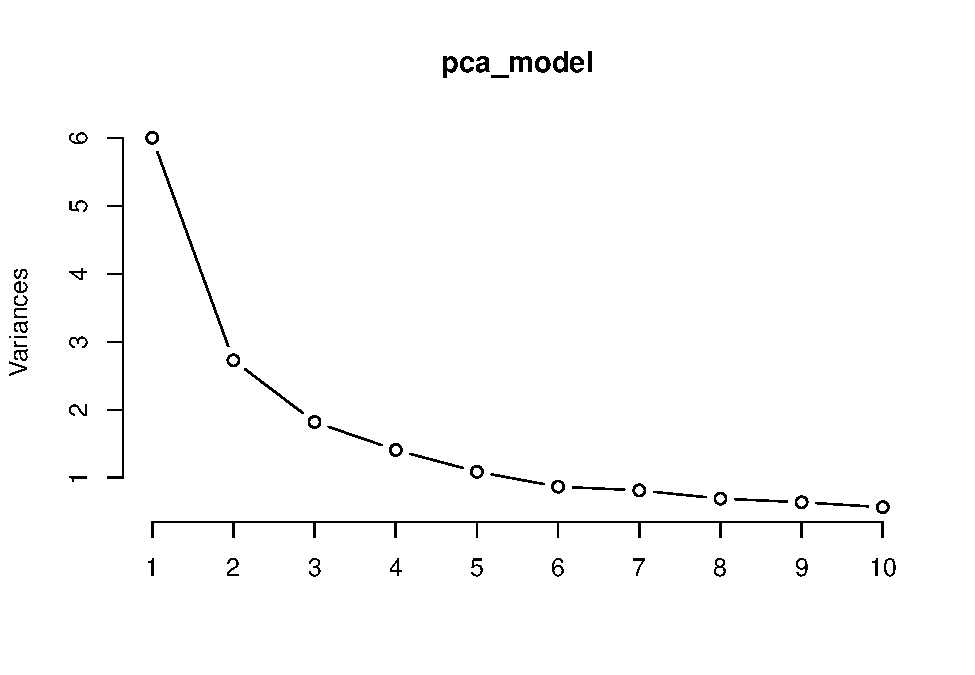
\includegraphics{583Project_files/figure-latex/unnamed-chunk-25-1.pdf}

\begin{Shaded}
\begin{Highlighting}[]
\CommentTok{\#str(le)}
\FunctionTok{class}\NormalTok{(df}\SpecialCharTok{$}\NormalTok{Country)}
\end{Highlighting}
\end{Shaded}

\begin{verbatim}
## [1] "NULL"
\end{verbatim}

\begin{Shaded}
\begin{Highlighting}[]
\NormalTok{glm\_model }\OtherTok{\textless{}{-}} \FunctionTok{glm}\NormalTok{(Life.expectancy}\SpecialCharTok{\textasciitilde{}}\NormalTok{., }\AttributeTok{data =}\NormalTok{ df, }\AttributeTok{family =} \StringTok{"gaussian"}\NormalTok{)}
\NormalTok{bic\_back }\OtherTok{\textless{}{-}} \FunctionTok{step}\NormalTok{(glm\_model, }\AttributeTok{k=}\FunctionTok{log}\NormalTok{(}\FunctionTok{nrow}\NormalTok{(df)), }\AttributeTok{direction=}\StringTok{"backward"}\NormalTok{, }\AttributeTok{trace=}\ConstantTok{FALSE}\NormalTok{)}
\FunctionTok{summary}\NormalTok{(bic\_back)}
\end{Highlighting}
\end{Shaded}

\begin{verbatim}
## 
## Call:
## glm(formula = Life.expectancy ~ Status + Adult.Mortality + infant.deaths + 
##     Hepatitis.B + BMI + under.five.deaths + Polio + Diphtheria + 
##     HIV.AIDS + thinness..1.19.years + Income.composition.of.resources + 
##     Schooling + GDP_scaled, family = "gaussian", data = df)
## 
## Deviance Residuals: 
##      Min        1Q    Median        3Q       Max  
## -21.1806   -2.1862   -0.1082    2.2527   18.3932  
## 
## Coefficients:
##                                   Estimate Std. Error t value Pr(>|t|)    
## (Intercept)                     56.0248606  0.6068087  92.327  < 2e-16 ***
## StatusDeveloping                -1.3992281  0.2465832  -5.674 1.54e-08 ***
## Adult.Mortality                 -0.0169017  0.0007858 -21.509  < 2e-16 ***
## infant.deaths                    0.0923034  0.0078837  11.708  < 2e-16 ***
## Hepatitis.B                     -0.0142558  0.0038221  -3.730 0.000195 ***
## BMI                              0.0404056  0.0048271   8.371  < 2e-16 ***
## under.five.deaths               -0.0692931  0.0058018 -11.943  < 2e-16 ***
## Polio                            0.0255695  0.0044766   5.712 1.24e-08 ***
## Diphtheria                       0.0331225  0.0047383   6.990 3.42e-12 ***
## HIV.AIDS                        -0.4819251  0.0168292 -28.636  < 2e-16 ***
## thinness..1.19.years            -0.0682138  0.0225535  -3.025 0.002513 ** 
## Income.composition.of.resources  6.4576087  0.6056113  10.663  < 2e-16 ***
## Schooling                        0.7678056  0.0395229  19.427  < 2e-16 ***
## GDP_scaled                       0.7397976  0.0918701   8.053 1.19e-15 ***
## ---
## Signif. codes:  0 '***' 0.001 '**' 0.01 '*' 0.05 '.' 0.1 ' ' 1
## 
## (Dispersion parameter for gaussian family taken to be 14.91597)
## 
##     Null deviance: 243118  on 2777  degrees of freedom
## Residual deviance:  41228  on 2764  degrees of freedom
## AIC: 15407
## 
## Number of Fisher Scoring iterations: 2
\end{verbatim}

\begin{Shaded}
\begin{Highlighting}[]
\FunctionTok{summary}\NormalTok{(glm\_model)}
\end{Highlighting}
\end{Shaded}

\begin{verbatim}
## 
## Call:
## glm(formula = Life.expectancy ~ ., family = "gaussian", data = df)
## 
## Deviance Residuals: 
##      Min        1Q    Median        3Q       Max  
## -21.6365   -2.1904   -0.0813    2.2726   18.6972  
## 
## Coefficients: (1 not defined because of singularities)
##                                   Estimate Std. Error t value Pr(>|t|)    
## (Intercept)                      1.366e+02  3.413e+01   4.003 6.41e-05 ***
## Year                            -4.046e-02  1.707e-02  -2.369 0.017888 *  
## StatusDeveloping                -1.340e+00  2.679e-01  -5.002 6.02e-07 ***
## Adult.Mortality                 -1.674e-02  7.966e-04 -21.011  < 2e-16 ***
## infant.deaths                    9.138e-02  8.101e-03  11.280  < 2e-16 ***
## Alcohol                         -2.433e-02  2.584e-02  -0.941 0.346621    
## Hepatitis.B                     -1.387e-02  3.833e-03  -3.617 0.000303 ***
## Measles                         -9.298e-06  8.300e-06  -1.120 0.262740    
## BMI                              3.946e-02  4.887e-03   8.074 1.01e-15 ***
## under.five.deaths               -6.807e-02  5.944e-03 -11.453  < 2e-16 ***
## Polio                            2.489e-02  4.482e-03   5.554 3.06e-08 ***
## Total.expenditure                5.942e-02  3.421e-02   1.737 0.082527 .  
## Diphtheria                       3.343e-02  4.749e-03   7.040 2.41e-12 ***
## HIV.AIDS                        -4.878e-01  1.705e-02 -28.609  < 2e-16 ***
## thinness..1.19.years            -7.134e-02  4.860e-02  -1.468 0.142241    
## thinness.5.9.years               6.001e-03  4.793e-02   0.125 0.900374    
## Income.composition.of.resources  6.736e+00  6.152e-01  10.949  < 2e-16 ***
## Schooling                        7.798e-01  4.083e-02  19.097  < 2e-16 ***
## Status.val                              NA         NA      NA       NA    
## GDP_scaled                       7.523e-01  9.195e-02   8.182 4.23e-16 ***
## Population_scaled               -6.306e-02  9.873e-02  -0.639 0.523086    
## ---
## Signif. codes:  0 '***' 0.001 '**' 0.01 '*' 0.05 '.' 0.1 ' ' 1
## 
## (Dispersion parameter for gaussian family taken to be 14.89595)
## 
##     Null deviance: 243118  on 2777  degrees of freedom
## Residual deviance:  41083  on 2758  degrees of freedom
## AIC: 15409
## 
## Number of Fisher Scoring iterations: 2
\end{verbatim}

\begin{Shaded}
\begin{Highlighting}[]
\FunctionTok{library}\NormalTok{(}\StringTok{"glmnet"}\NormalTok{)}
\end{Highlighting}
\end{Shaded}

\begin{verbatim}
## Warning: package 'glmnet' was built under R version 4.2.2
\end{verbatim}

\begin{verbatim}
## Loading required package: Matrix
\end{verbatim}

\begin{verbatim}
## Warning: package 'Matrix' was built under R version 4.2.2
\end{verbatim}

\begin{verbatim}
## 
## Attaching package: 'Matrix'
\end{verbatim}

\begin{verbatim}
## The following objects are masked from 'package:tidyr':
## 
##     expand, pack, unpack
\end{verbatim}

\begin{verbatim}
## Loaded glmnet 4.1-6
\end{verbatim}

\begin{Shaded}
\begin{Highlighting}[]
\CommentTok{\#head(df\_ns) \#using non{-}scaled GDP and Population}
\NormalTok{df\_ns}\SpecialCharTok{$}\NormalTok{Status }\OtherTok{\textless{}{-}} \FunctionTok{as.numeric}\NormalTok{(}\FunctionTok{as.factor}\NormalTok{(df\_ns}\SpecialCharTok{$}\NormalTok{Status)) }\CommentTok{\#Convert Non{-}Numeric Columns to Numeric for glmnet}
\NormalTok{y }\OtherTok{\textless{}{-}}\NormalTok{ df\_ns}\SpecialCharTok{$}\NormalTok{Life.expectancy}
\NormalTok{x }\OtherTok{\textless{}{-}} \FunctionTok{as.matrix}\NormalTok{(df\_ns[,}\FunctionTok{c}\NormalTok{(}\SpecialCharTok{{-}}\DecValTok{1}\NormalTok{,}\SpecialCharTok{{-}}\DecValTok{3}\NormalTok{)])}

\NormalTok{grid }\OtherTok{\textless{}{-}} \FunctionTok{exp}\NormalTok{(}\FunctionTok{seq}\NormalTok{(}\DecValTok{2}\NormalTok{, }\SpecialCharTok{{-}}\DecValTok{9}\NormalTok{, }\AttributeTok{length=}\DecValTok{100}\NormalTok{)) }

\NormalTok{ladf}\OtherTok{\textless{}{-}} \FunctionTok{cv.glmnet}\NormalTok{(x, y, }\AttributeTok{alpha=}\DecValTok{1}\NormalTok{, }\AttributeTok{lambda=}\NormalTok{grid, }\AttributeTok{standardize =} \ConstantTok{TRUE}\NormalTok{)}
\FunctionTok{plot}\NormalTok{(ladf}\SpecialCharTok{$}\NormalTok{glmnet.fit, }\AttributeTok{label=}\ConstantTok{TRUE}\NormalTok{, }\AttributeTok{xvar=}\StringTok{"lambda"}\NormalTok{)}
\end{Highlighting}
\end{Shaded}

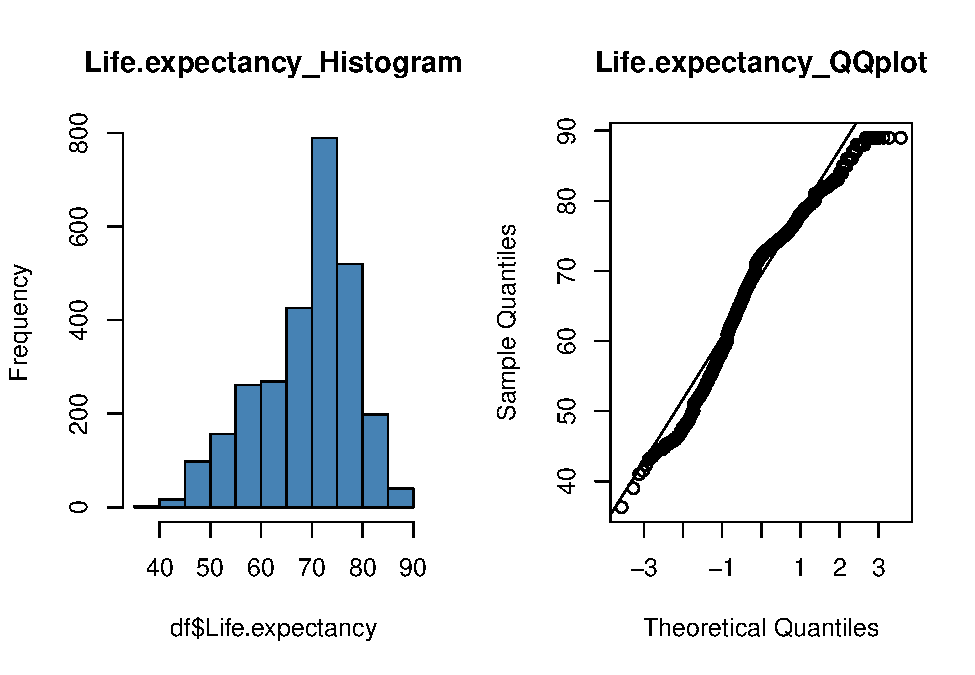
\includegraphics{583Project_files/figure-latex/unnamed-chunk-27-1.pdf}

\begin{Shaded}
\begin{Highlighting}[]
\FunctionTok{plot}\NormalTok{(ladf)}
\end{Highlighting}
\end{Shaded}

\includegraphics{583Project_files/figure-latex/unnamed-chunk-27-2.pdf}

\begin{Shaded}
\begin{Highlighting}[]
\FunctionTok{coef}\NormalTok{(ladf) }\CommentTok{\#thinness.5.9.years is removed since the coefficients went to 0}
\end{Highlighting}
\end{Shaded}

\begin{verbatim}
## 20 x 1 sparse Matrix of class "dgCMatrix"
##                                            s1
## (Intercept)                      5.566793e+01
## Status                          -1.225671e+00
## Adult.Mortality                 -1.723016e-02
## infant.deaths                    2.391887e-02
## Alcohol                         -2.407424e-02
## Hepatitis.B                     -1.409929e-02
## Measles                         -1.165208e-05
## BMI                              3.978760e-02
## under.five.deaths               -1.864634e-02
## Polio                            2.669657e-02
## Total.expenditure                4.227257e-02
## Diphtheria                       3.659660e-02
## HIV.AIDS                        -4.877876e-01
## GDP                              4.894765e-05
## Population                       4.542322e-10
## thinness..1.19.years            -5.241728e-02
## thinness.5.9.years               .           
## Income.composition.of.resources  7.012347e+00
## Schooling                        7.814078e-01
## Status.val                       4.051386e-02
\end{verbatim}

\begin{Shaded}
\begin{Highlighting}[]
\FunctionTok{library}\NormalTok{(}\StringTok{"glmnet"}\NormalTok{)}
\NormalTok{df}\SpecialCharTok{$}\NormalTok{Status }\OtherTok{\textless{}{-}} \FunctionTok{as.numeric}\NormalTok{(}\FunctionTok{as.factor}\NormalTok{(df}\SpecialCharTok{$}\NormalTok{Status)) }\CommentTok{\#Convert Non{-}Numeric Columns to Numeric for glmnet}
\NormalTok{y }\OtherTok{\textless{}{-}}\NormalTok{ df}\SpecialCharTok{$}\NormalTok{Life.expectancy}
\NormalTok{x }\OtherTok{\textless{}{-}} \FunctionTok{as.matrix}\NormalTok{(df[,}\FunctionTok{c}\NormalTok{(}\SpecialCharTok{{-}}\DecValTok{1}\NormalTok{,}\SpecialCharTok{{-}}\DecValTok{3}\NormalTok{)])}
\NormalTok{grid }\OtherTok{\textless{}{-}} \FunctionTok{exp}\NormalTok{(}\FunctionTok{seq}\NormalTok{(}\DecValTok{2}\NormalTok{, }\SpecialCharTok{{-}}\DecValTok{9}\NormalTok{, }\AttributeTok{length=}\DecValTok{100}\NormalTok{)) }

\NormalTok{ladf}\OtherTok{\textless{}{-}} \FunctionTok{cv.glmnet}\NormalTok{(x, y, }\AttributeTok{alpha=}\DecValTok{1}\NormalTok{, }\AttributeTok{lambda=}\NormalTok{grid, }\AttributeTok{standardize =} \ConstantTok{TRUE}\NormalTok{)}

\FunctionTok{plot}\NormalTok{(ladf}\SpecialCharTok{$}\NormalTok{glmnet.fit, }\AttributeTok{label=}\ConstantTok{TRUE}\NormalTok{, }\AttributeTok{xvar=}\StringTok{"lambda"}\NormalTok{)}
\end{Highlighting}
\end{Shaded}

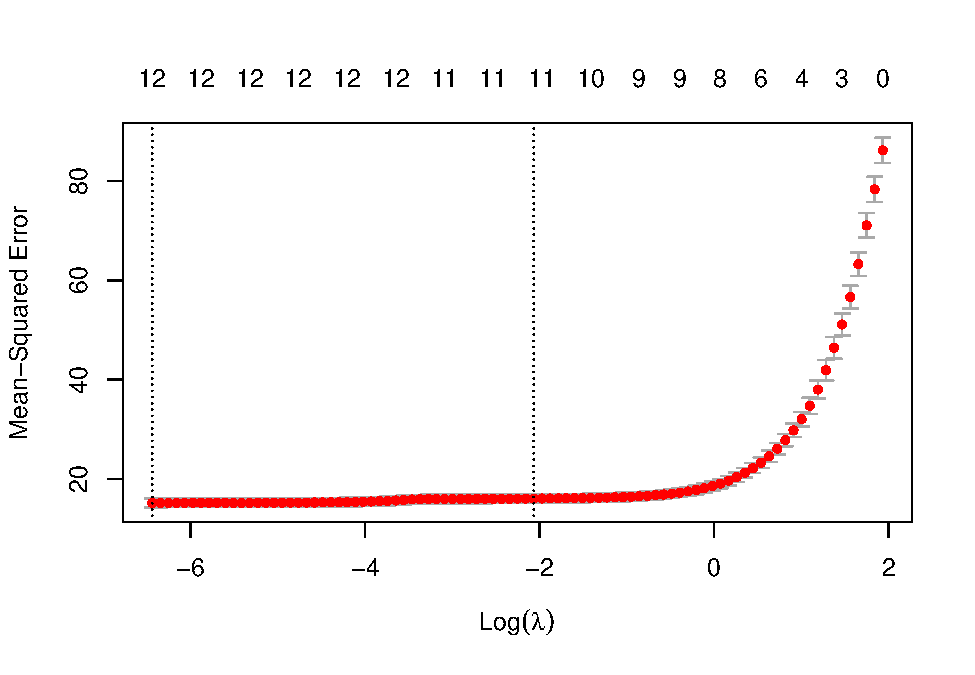
\includegraphics{583Project_files/figure-latex/unnamed-chunk-28-1.pdf}

\begin{Shaded}
\begin{Highlighting}[]
\FunctionTok{plot}\NormalTok{(ladf)}
\end{Highlighting}
\end{Shaded}

\includegraphics{583Project_files/figure-latex/unnamed-chunk-28-2.pdf}

\begin{Shaded}
\begin{Highlighting}[]
\FunctionTok{coef}\NormalTok{(ladf)}
\end{Highlighting}
\end{Shaded}

\begin{verbatim}
## 20 x 1 sparse Matrix of class "dgCMatrix"
##                                            s1
## (Intercept)                      5.592775e+01
## Status                          -1.213783e+00
## Adult.Mortality                 -1.726463e-02
## infant.deaths                    1.637326e-02
## Alcohol                         -2.490441e-02
## Hepatitis.B                     -1.406696e-02
## Measles                         -1.201192e-05
## BMI                              3.980534e-02
## under.five.deaths               -1.311626e-02
## Polio                            2.682963e-02
## Total.expenditure                4.125993e-02
## Diphtheria                       3.698714e-02
## HIV.AIDS                        -4.883208e-01
## thinness..1.19.years            -5.064999e-02
## thinness.5.9.years               .           
## Income.composition.of.resources  7.067575e+00
## Schooling                        7.826532e-01
## Status.val                       3.707533e-02
## GDP_scaled                       6.937109e-01
## Population_scaled                3.772243e-02
\end{verbatim}

\#\#\#\#\#\#\#\#\#\#\#\#\#\#\#PCA(suggest a simpler scoring
system):\#\#\#\#\#\#\#\#\#\#\#\#\#\#\#\#\#\#\#\#\#\#\#\#\#\#
\#\#\#\#\#\#\#\#\#\#\#\#\#\#\#\#\#\#\#\#\#\#\#\#\#\#\#\#\#\#\#\#\#\#\#\#\#\#\#\#\#\#\#\#\#\#\#\#\#\#\#\#\#\#\#\#\#\#\#\#\#\#\#\#\#\#\#\#\#\#\#\#\#\#\#\#\#\#\#

\begin{Shaded}
\begin{Highlighting}[]
\CommentTok{\#head(df[,{-}3])}
\FunctionTok{head}\NormalTok{(df[,}\FunctionTok{c}\NormalTok{(}\SpecialCharTok{{-}}\DecValTok{1}\NormalTok{,}\SpecialCharTok{{-}}\DecValTok{3}\NormalTok{)])}
\end{Highlighting}
\end{Shaded}

\begin{verbatim}
##   Status Adult.Mortality infant.deaths Alcohol Hepatitis.B Measles  BMI
## 1      2             263            62    0.01          65    1154 19.1
## 2      2             271            64    0.01          62     492 18.6
## 3      2             268            66    0.01          64     430 18.1
## 4      2             272            69    0.01          67    2787 17.6
## 5      2             275            71    0.01          68    3013 17.2
## 6      2             279            74    0.01          66    1989 16.7
##   under.five.deaths Polio Total.expenditure Diphtheria HIV.AIDS
## 1                83     6              8.16         65      0.1
## 2                86    58              8.18         62      0.1
## 3                89    62              8.13         64      0.1
## 4                93    67              8.52         67      0.1
## 5                97    68              7.87         68      0.1
## 6               102    66              9.20         66      0.1
##   thinness..1.19.years thinness.5.9.years Income.composition.of.resources
## 1                 17.2               17.3                           0.479
## 2                 17.5               17.5                           0.476
## 3                 17.7               17.7                           0.470
## 4                 17.9               18.0                           0.463
## 5                 18.2               18.2                           0.454
## 6                 18.4               18.4                           0.448
##   Schooling Status.val GDP_scaled Population_scaled
## 1      10.1          0 -0.4834490         0.3439174
## 2      10.0          0 -0.4814562        -0.2036611
## 3       9.9          0 -0.4801214         0.3110582
## 4       9.8          0 -0.4774435        -0.1484364
## 5       9.5          0 -0.5199393        -0.1602105
## 6       9.2          0 -0.4856165        -0.1617746
\end{verbatim}

\begin{Shaded}
\begin{Highlighting}[]
\NormalTok{df}\SpecialCharTok{$}\NormalTok{Status }\OtherTok{\textless{}{-}} \FunctionTok{as.numeric}\NormalTok{(}\FunctionTok{as.factor}\NormalTok{(df}\SpecialCharTok{$}\NormalTok{Status)) }\CommentTok{\#Convert Non{-}Numeric Columns to Numeric for PCA}
\NormalTok{pca\_model }\OtherTok{\textless{}{-}} \FunctionTok{prcomp}\NormalTok{(df[,}\FunctionTok{c}\NormalTok{(}\SpecialCharTok{{-}}\DecValTok{1}\NormalTok{,}\SpecialCharTok{{-}}\DecValTok{3}\NormalTok{)],}\AttributeTok{scale.=}\ConstantTok{TRUE}\NormalTok{)}
\FunctionTok{summary}\NormalTok{(pca\_model)}
\end{Highlighting}
\end{Shaded}

\begin{verbatim}
## Importance of components:
##                           PC1    PC2     PC3     PC4     PC5     PC6     PC7
## Standard deviation     2.4508 1.6521 1.34948 1.18718 1.04354 0.93214 0.90244
## Proportion of Variance 0.3161 0.1436 0.09585 0.07418 0.05732 0.04573 0.04286
## Cumulative Proportion  0.3161 0.4598 0.55562 0.62980 0.68711 0.73284 0.77570
##                            PC8     PC9   PC10    PC11    PC12    PC13    PC14
## Standard deviation     0.83225 0.79978 0.7525 0.70967 0.69730 0.64848 0.62733
## Proportion of Variance 0.03646 0.03367 0.0298 0.02651 0.02559 0.02213 0.02071
## Cumulative Proportion  0.81216 0.84582 0.8756 0.90213 0.92772 0.94986 0.97057
##                           PC15    PC16    PC17    PC18      PC19
## Standard deviation     0.55150 0.43756 0.24635 0.05344 4.246e-14
## Proportion of Variance 0.01601 0.01008 0.00319 0.00015 0.000e+00
## Cumulative Proportion  0.98658 0.99666 0.99985 1.00000 1.000e+00
\end{verbatim}

\begin{Shaded}
\begin{Highlighting}[]
\CommentTok{\#Use Sceen Plot to decide how many PC to keep, But there seems to be a large value in our PC1 Standard Deviation so it isn\textquotesingle{}t a clear indicator.}

\FunctionTok{plot}\NormalTok{(pca\_model, }\AttributeTok{type=}\StringTok{"lines"}\NormalTok{)}
\end{Highlighting}
\end{Shaded}

\includegraphics{583Project_files/figure-latex/unnamed-chunk-30-1.pdf}

\begin{Shaded}
\begin{Highlighting}[]
\CommentTok{\#Use Standard deviation instead to decide how many PC to keep, if it is below 1 we toss it out since it does not explain much info about our data.it is suggest us to keep 15 PC.}

\NormalTok{pca\_model}\SpecialCharTok{$}\NormalTok{rotation[,}\DecValTok{1}\SpecialCharTok{:}\DecValTok{15}\NormalTok{]}
\end{Highlighting}
\end{Shaded}

\begin{verbatim}
##                                         PC1          PC2          PC3
## Status                          -0.27840223 -0.220313018  0.258436562
## Adult.Mortality                 -0.21142385 -0.162226887 -0.158840956
## infant.deaths                   -0.20029744  0.483274049  0.022797136
## Alcohol                          0.24451808  0.158125047 -0.232907482
## Hepatitis.B                      0.12174403 -0.045765085  0.460153365
## Measles                         -0.12960468  0.326890529 -0.013181845
## BMI                              0.26533516  0.021993522  0.023040962
## under.five.deaths               -0.20485162  0.478174505  0.007792975
## Polio                            0.20517076  0.048738683  0.457638500
## Total.expenditure                0.14300395  0.008430669 -0.137236721
## Diphtheria                       0.20683732  0.045387397  0.489651141
## HIV.AIDS                        -0.12960010 -0.107185001 -0.194076591
## thinness..1.19.years            -0.30251693  0.147167753  0.155837376
## thinness.5.9.years              -0.30205344  0.150075505  0.153347479
## Income.composition.of.resources  0.30146577  0.171094423  0.061792724
## Schooling                        0.32068256  0.154490286  0.040360612
## Status.val                       0.27840223  0.220313018 -0.258436562
## GDP_scaled                       0.21889362  0.151445679 -0.104763843
## Population_scaled               -0.09940392  0.379091667  0.063278260
##                                         PC4         PC5           PC6
## Status                          -0.26171826 -0.26585381  0.1978906383
## Adult.Mortality                  0.41011167 -0.24773789  0.1878883402
## infant.deaths                   -0.04442242 -0.14578324 -0.0167980763
## Alcohol                          0.21125069 -0.14666302 -0.0039724933
## Hepatitis.B                      0.26258039 -0.02296182 -0.2760673704
## Measles                         -0.05860130 -0.20437955 -0.3106057832
## BMI                             -0.26883812 -0.27016994  0.1936575638
## under.five.deaths               -0.03925740 -0.14778587 -0.0282887815
## Polio                            0.20870648 -0.09165746  0.0240406145
## Total.expenditure                0.16902597 -0.43251203 -0.4029172353
## Diphtheria                       0.22056183 -0.11358764  0.0006524693
## HIV.AIDS                         0.50779133 -0.31294996  0.3802851712
## thinness..1.19.years             0.22768814  0.31774605  0.0814517665
## thinness.5.9.years               0.23236037  0.31776225  0.0951979998
## Income.composition.of.resources -0.06881819  0.03931768  0.3711272957
## Schooling                       -0.01761425 -0.02612192  0.3074863751
## Status.val                       0.26171826  0.26585381 -0.1978906383
## GDP_scaled                       0.06192637  0.25536069  0.2420481857
## Population_scaled               -0.09314302 -0.20419514  0.2469428120
##                                          PC7         PC8         PC9
## Status                          -0.056989927 -0.20489122  0.03009121
## Adult.Mortality                  0.151844198  0.16271840  0.07409489
## infant.deaths                    0.008922021  0.03300675  0.02276178
## Alcohol                          0.115353795  0.04517767 -0.30623201
## Hepatitis.B                      0.227935624  0.07651286  0.14097281
## Measles                          0.461761130 -0.50858125 -0.03920852
## BMI                             -0.027793919 -0.01912920  0.02422345
## under.five.deaths                0.021247173  0.02570310  0.02518330
## Polio                           -0.002589591  0.02519473  0.01815921
## Total.expenditure               -0.708206450 -0.21422323  0.10854800
## Diphtheria                       0.018879327  0.04343499  0.02272697
## HIV.AIDS                         0.129387839 -0.17378131  0.02137230
## thinness..1.19.years            -0.270910825 -0.15428933 -0.13773796
## thinness.5.9.years              -0.265158966 -0.15209428 -0.16310944
## Income.composition.of.resources -0.060437508 -0.19619131 -0.25708521
## Schooling                       -0.076909357 -0.18318758 -0.29715424
## Status.val                       0.056989927  0.20489122 -0.03009121
## GDP_scaled                      -0.001460450 -0.34132170  0.78260475
## Population_scaled               -0.136846812  0.55389147  0.22415494
##                                        PC10        PC11         PC12
## Status                          -0.01590129  0.22110421 -0.167656922
## Adult.Mortality                  0.01536016 -0.06553883 -0.309850800
## infant.deaths                    0.10950707 -0.18088031 -0.243123063
## Alcohol                         -0.05833326  0.43360711 -0.508716200
## Hepatitis.B                      0.66033820  0.27231132  0.050442295
## Measles                         -0.17450839  0.08077685  0.300740238
## BMI                              0.40769358 -0.52860334 -0.057568050
## under.five.deaths                0.11577772 -0.17869282 -0.253891871
## Polio                           -0.47369074 -0.28051749 -0.075821619
## Total.expenditure                0.02259966  0.07117627  0.062235193
## Diphtheria                      -0.25031929 -0.06671621 -0.055967896
## HIV.AIDS                         0.08126877 -0.13070955  0.381045057
## thinness..1.19.years             0.09847767 -0.02756391  0.002423892
## thinness.5.9.years               0.09197419 -0.01582999 -0.017358528
## Income.composition.of.resources  0.09999330  0.11701572  0.104251647
## Schooling                        0.07732531  0.15546282  0.084270615
## Status.val                       0.01590129 -0.22110421  0.167656922
## GDP_scaled                      -0.03240781  0.13201456 -0.198620681
## Population_scaled               -0.09166408  0.35153238  0.391704393
##                                          PC13        PC14          PC15
## Status                           0.0002459252 -0.07026207  0.0223017011
## Adult.Mortality                  0.0608782285  0.68774207  0.0741522261
## infant.deaths                   -0.2962823882 -0.08373777 -0.0002152361
## Alcohol                          0.3344873945 -0.33075376 -0.0213033209
## Hepatitis.B                     -0.0583789421 -0.01962561  0.1769038325
## Measles                          0.2865157091  0.22586611 -0.0005600566
## BMI                              0.5376965282 -0.01387673 -0.0642163849
## under.five.deaths               -0.2922848678 -0.09122794  0.0059996616
## Polio                            0.0679038676 -0.11037186  0.6040881233
## Total.expenditure               -0.0395632946  0.09992181  0.0275969220
## Diphtheria                      -0.0394077715  0.05596770 -0.7585554714
## HIV.AIDS                        -0.1326213062 -0.44350091 -0.0484421376
## thinness..1.19.years             0.2832060950  0.01017193 -0.0095964810
## thinness.5.9.years               0.2560970686  0.01735304 -0.0239073013
## Income.composition.of.resources -0.2870410309  0.29465811  0.0520053779
## Schooling                       -0.1229666739  0.16982177  0.0976061537
## Status.val                      -0.0002459252  0.07026207 -0.0223017011
## GDP_scaled                       0.0489259246 -0.01684190 -0.0042997455
## Population_scaled                0.2560570655  0.04968566  0.0353137863
\end{verbatim}

\#\#\#\#\#\#\#\#\#\#\#\#\#\#\#\#\#\#\#\#\#\#\#\#\#\#\#\#\#\#\#\#\#\#\#\#\#\#\#\#\#FA:(not
working)\#\#\#\#\#\#\#\#\#\#\#\#\#\#\#\#\#\#\#\#\#\#\#\#\#\#\#\#\#\#\#\#\#\#\#
\#\#\#\#\#\#\#\#\#\#\#\#\#\#\#\#\#\#\#\#\#\#\#\#\#\#\#\#\#\#\#\#\#\#\#\#\#\#\#\#\#\#\#\#\#\#\#\#\#\#\#\#\#\#\#\#\#\#\#\#\#\#\#\#\#\#\#\#\#\#\#\#\#\#\#\#\#\#\#

df2 = subset(le\_dropped, select =
-c(Country,GDP\_scaled,Population\_scaled) ) head(df2)

head(df) fa\_model \textless- factanal(df2, factors = 13)

\end{document}
